% =====================================================================
%  Full_Thesis_Report.tex
%  Preamble and structure matched to the departmental example report.
%  Compile on Overleaf with pdfLaTeX. Run TWICE so the ToC resolves.
%
%  TO DO BEFORE SUBMITTING:
%   1. Put the university logo in  images/university logo.jpg
%   2. Confirm the Session line on the title page (currently 2020-21)
%   3. Complete references [4] and [6] (see README.txt)
% =====================================================================
\documentclass[12pt,a4paper]{report}
\usepackage[left=1.2in,right=0.8in,top=1in,bottom=1in]{geometry}
\usepackage{times}
\usepackage{setspace}
\usepackage{graphicx}
\usepackage{array}
\usepackage{longtable}
\usepackage{booktabs}
\usepackage{amsmath}
\usepackage{amsfonts}
\usepackage{amssymb}
\usepackage{fancyhdr}
\usepackage{titlesec}
\usepackage{tocloft}
\usepackage[hidelinks]{hyperref}
\usepackage[english]{babel}
\usepackage{ragged2e}
\usepackage{parskip}

\renewcommand{\rmdefault}{ptm}

\onehalfspacing

\titleformat{\chapter}[display]
{\normalfont\fontsize{16}{19}\bfseries\centering}
{\chaptertitlename\ \thechapter}{20pt}{\fontsize{16}{19}\bfseries\uppercase}

\titleformat{\section}
{\normalfont\fontsize{14}{17}\bfseries}{\thesection}{1em}{}

\titleformat{\subsection}
{\normalfont\fontsize{12}{15}\bfseries}{\thesubsection}{1em}{}

\pagenumbering{roman}

\begin{document}

% ========================= TITLE PAGE ================================
\begin{titlepage}
\centering
\vspace*{0.5cm}


\includegraphics[width=2.5cm]{images/university logo.jpg}
\vspace{0.5cm}

{\fontsize{17}{21}\bfseries
A LIGHTWEIGHT, TRAINING-FREE, RELIABILITY-AWARE GEOMETRIC CANONICALIZATION FRAMEWORK FOR CROSS-VIEW COMPARABILITY OF FROZEN MONOCULAR 3D POSE PREDICTIONS
}
\vspace{0.7cm}

{\fontsize{14}{17}\selectfont
A PROJECT REPORT
}
\vspace{0.4cm}

{\fontsize{14}{17}\selectfont
Submitted by
}
\vspace{0.4cm}

{\fontsize{16}{19}\selectfont\itshape
MEHEDI HASAN KHAN
}
\vspace{0.3cm}

{\fontsize{14}{17}\selectfont
ID: 12108004
}
\vspace{0.3cm}

{\fontsize{14}{17}\selectfont
Session: 2020-21
}
\vspace{0.6cm}

{\fontsize{14}{18}\itshape in partial fulfillment for the award of the degree of\par}
    \vspace{0.4cm}

    {\fontsize{16}{20} BACHELOR OF SCIENCE IN COMPUTER SCIENCE AND ENGINEERING\par}
    \vspace{0.4cm}

    {\fontsize{14}{18} IN\par}
    \vspace{0.4cm}

    {\fontsize{14}{18} DEPARTMENT OF COMPUTER SCIENCE AND ENGINEERING\par}
    \vspace{0.6cm}

    {\fontsize{16}{20} COMILLA UNIVERSITY :: COMILLA-3506\par}
    \vspace{0.8cm}

    {\fontsize{14}{18} August 2026\par}

\end{titlepage}

% ===================== BONAFIDE CERTIFICATE ==========================
\newpage
\thispagestyle{empty}
\begin{center}
{\fontsize{18}{22}\bfseries
COMILLA UNIVERSITY :: COMILLA-3506
}
\vspace{1cm}

{\fontsize{16}{19}\bfseries
BONAFIDE CERTIFICATE
}
\end{center}
\vspace{2cm}

\doublespacing
{\fontsize{14}{17}\selectfont
Certified that this project report ``A Lightweight, Training-Free, Reliability-Aware Geometric Canonicalization Framework for Cross-View Comparability of Frozen Monocular 3D Pose Predictions'' is the bonafide work of ``MEHEDI HASAN KHAN'' who carried out the project work under my supervision.
}
\vspace{3cm}

\begin{center}
% The two department lines are the widest cells and together overran the text
% block by 41pt at the default 12pt, leaving no gap between the columns. The
% table sits outside the 14pt group above, so it was already at 12; 11 is what
% actually brings it inside the margins.
{\fontsize{11}{13}\selectfont
 \begin{tabular}{cc}
        \underline{\hspace{5.6cm}} & \underline{\hspace{5.6cm}} \\
        \textbf{SIGNATURE} & \textbf{SIGNATURE} \\
        \textbf{Dr. Md. Faisal Bin Abdul Aziz} & \textbf{Dr. Mahmudul Hasan} \\
        Chairman, Exam Committee & Supervisor \\
        Associate Professor & Associate Professor \\
        Department of Computer Science \& Engineering & Department of Computer Science \& Engineering \\
        Comilla University, Cumilla & Comilla University, Cumilla \\
    \end{tabular}}
\end{center}

% ============================ ABSTRACT ===============================
\newpage
\setcounter{page}{3}
\chapter*{ABSTRACT}
\addcontentsline{toc}{chapter}{ABSTRACT}

\doublespacing
{\fontsize{12}{15}\selectfont
Monocular 3D human pose estimators produce skeletons expressed in the coordinate frame of the observing camera, so the same motion recorded from two viewpoints yields two different sets of coordinates, which prevents direct comparison in applications such as gait analysis and sports science. However, existing remedies either retrain the estimator, require camera calibration, or learn a canonicalization network, and all assume access to training data. In this project we present a framework that adds no trained parameters to a frozen, off-the-shelf estimator. We construct a body-fixed coordinate frame from anatomical axes by Gram-Schmidt orthonormalization, apply it after prediction, and extend it to one frame per limb. We evaluate on two datasets. On MPI-INF-3DHP, canonicalization reduces cross-view joint distance by 32.4 percent over twenty-seven held-out camera pairs, and the resulting distance tracks true prediction error at a Spearman coefficient of 0.601 against 0.188 for the raw distance. On Human3.6M, which played no part in developing the method so that all 180 camera pairs are held out, it reduces cross-view distance by 74.1 percent, improves 179 of the 180 pairs, and closes 90.5 percent of the gap to a per-frame Procrustes oracle that requires both views at once. We also report the failures. An analytic reliability score is falsified as a predictor of accuracy along seven independent axes, and a temporal bone-length signal that reaches a coefficient of 0.492 on the first dataset falls to 0.098 on the second, so we retract it. Both failures share one cause: geometric plausibility is invariant to the coherent depth error that dominates monocular estimation.
}

% ========================= ACKNOWLEDGEMENT ===========================
\newpage
\chapter*{ACKNOWLEDGEMENT}
\addcontentsline{toc}{chapter}{ACKNOWLEDGEMENT}

\justifying
{\fontsize{12pt}{15pt}\selectfont
I would like to express my deepest gratitude to my project supervisor, \textbf{Dr. Mahmudul Hasan}, for his invaluable guidance, continuous support, and patience throughout this project. His critical feedback shaped this work substantially: an early evaluation was found to rest on an invalid protocol, and the requirement to justify every claim against evidence led directly to the corrected methodology and the audited reporting practice adopted here. I am also thankful to the Department of Computer Science and Engineering, Comilla University, for providing the necessary resources and infrastructure. My sincere thanks to the examination committee for their valuable suggestions and feedback. Special thanks to my family and friends for their constant support and motivation during this project work.
}

\newpage
\tableofcontents

\newpage
\listoffigures

\newpage
\listoftables

\newpage
\pagenumbering{arabic}
\onehalfspacing

% ========================== CHAPTER 1 ================================
\chapter{INTRODUCTION}

\section{Background}

Three-dimensional human pose estimation recovers the spatial coordinates of body joints from visual input. Depth sensors and calibrated multi-camera rigs achieve high accuracy, but their cost and setup requirements make them impractical for deployment outside the laboratory. Monocular estimation from ordinary RGB video is therefore of considerable practical interest, and modern transformer-based lifting networks such as MotionAGFormer [1] and MotionBERT [2] achieve mean per-joint position errors near 45 mm on the Human3.6M benchmark [11].

These estimators share a property that limits their use in comparative analysis. The predicted skeleton is expressed relative to the observing camera, so two cameras viewing the same subject at the same instant produce two different sets of coordinates for the same physical pose. Any application that compares poses across viewpoints, such as gait analysis across sessions, sports analytics across camera positions, or multi-device capture, must first reconcile those coordinate frames.

\section{Motivation}

Three practical constraints motivate the approach taken in this project. First, practitioners frequently cannot retrain the estimator: it is a third-party artifact, the deployment data has no labels, and the computational budget for training is unavailable. Second, camera calibration is often impossible, as in footage recorded by uncontrolled devices. Third, and least addressed in the literature, a system that silently produces a wrong pose is more dangerous than one that declines to answer, so a deployable framework should indicate when its own output should not be trusted.

\section{Objectives}

The main objectives of this project are:

\begin{itemize}
\item \textbf{Construct a viewpoint-independent coordinate frame}: remove camera-induced orientation variation from the output of a frozen monocular estimator without training, labels, or camera parameters.

\item \textbf{Estimate prediction reliability analytically}: score individual predictions using geometric quantities alone, and abstain when reliability is low.

\item \textbf{Evaluate under an auditable protocol}: design an evaluation free of the methodological defects identified in earlier work, with every reported number recomputed from stored artifacts.

\item \textbf{Characterize failure honestly}: identify the conditions under which the proposed signals do not work, and explain why.
\end{itemize}

\section{Contributions}

\begin{itemize}
\item A canonicalization and reliability framework that adds zero learned parameters to a frozen estimator, evaluated over 209 camera pairs across two datasets and, without a line of code changed, over a second backbone nineteen times larger and of a different architecture family.

\item A cross-dataset replication of the central claim on Human3.6M, where canonicalization improves 179 of 180 held-out camera pairs and closes 90.5 percent of the gap to a per-frame Procrustes oracle.

\item A multi-scale extension constructing one body frame per limb, improving cross-view consistency on all twenty-nine MPI-INF-3DHP pairs and on 179 of the 180 held-out Human3.6M pairs, together with the finding that the length of the axis a frame is built from governs its cross-view consistency. Rebuilding every segment frame from that segment's own long axis raises the improvement from 25.6 to 55.1 percent and improves all 180 pairs.

\item Calibration-free multi-view fusion in the shared frame, together with the finding that the estimator must be robust when views are few, since at four views a median reliably improves on an arbitrary single view while an unweighted mean does not.

\item A systematic falsification of the proposed quality signal along five independent axes, and identification of its underlying cause.

\item A cross-dataset replication that retracts our own bone-length error predictor and bounds the condition under which it holds.
\end{itemize}

\section{Report Organization}

Chapter 2 reviews related work and positions this project against it. Chapter 3 describes the methodology. Chapter 4 describes the two datasets, the joint conventions that connect them, and the implemented system. Chapter 5 presents the experimental protocol and results, including the negative results and one retraction. Chapter 6 concludes and identifies future work. Appendix A contains the complete result tables, generated directly from the stored artifacts.

% ========================== CHAPTER 2 ================================
\chapter{LITERATURE REVIEW}

Cross-view comparability of 3D human pose has been approached from several directions, and the methods differ less in accuracy than in what they require at deployment time. This chapter reviews the relevant literature and states precisely where the present work sits.

\section{Monocular 3D Pose Estimation}

Contemporary monocular pipelines follow a two-stage design in which a 2D keypoint detector locates joints in the image and a lifting network maps the 2D sequence to 3D coordinates. The division persists because the two stages fail differently: detection fails on occlusion and motion blur, while lifting fails on depth ambiguity, and a single network trained end to end obscures which of the two is responsible for a given error.

\subsection{Two-Dimensional Detection}

The first stage is mature. Stacked hourglass networks [12] established the repeated downsampling and upsampling design that most later detectors adopt, and modern single-stage detectors such as YOLOv8 [13] reach comparable keypoint accuracy at real-time speed. The choice matters to this project only through the quality of what reaches the lifting network. Human3.6M results in the literature are conventionally reported using stacked hourglass detections, while a deployment on arbitrary footage uses a general detector; we use the former on Human3.6M and the latter on MPI-INF-3DHP, and the difference is one of the conditions that changes between our two evaluations.

\subsection{Lifting Two-Dimensional Keypoints to Three Dimensions}

Martinez et al. [14] showed that a network of two residual blocks, given ground-truth 2D keypoints, outperformed contemporary systems that consumed the image directly. The result established that most of the difficulty in monocular 3D pose is the ambiguity of the lifting problem rather than the extraction of image features, and it made the two-stage design the default.

Single-frame lifting is nevertheless ill-posed, since infinitely many 3D configurations project to the same 2D observation. Temporal context resolves much of this ambiguity, and the field moved to sequence models accordingly. Pavllo et al. [15] used dilated temporal convolutions over a window of frames. MotionBERT [2] applies a dual-stream spatio-temporal transformer with heterogeneous pretraining. MotionAGFormer [1] combines a transformer stream, which captures long-range dependence, with a graph-convolutional stream that respects the skeleton's connectivity, and reaches 45.1 mm mean per-joint position error on Human3.6M with 2.2 million parameters. We use the extra-small variant of that architecture as a frozen component throughout.

Two observations from this literature bear directly on the present work. First, the reported accuracies are averages over an in-domain test split, and per-action figures vary by a factor of two, with seated actions consistently worst. Second, none of these architectures produces an output whose coordinate frame is comparable across cameras, because each predicts in the frame of the observing camera. Accuracy and comparability are separate properties, and progress on the first has not delivered the second.

\section{Canonicalization and View-Invariant Representations}

\noindent \textbf{Comparison of Proposed System vs Existing Systems}

\vspace{0.5cm}

\noindent \textbf{Author:} Ekanayake et al. (2025) \\
\textbf{Method:} 3DPCNet, estimator-agnostic canonicalization of 3D pose \\
\textbf{Focus (Solved Issues):} Predicts a 6D rotation to rectify camera-centred skeletons, operating directly on 3D joint coordinates \\
\textbf{Methodology:} Graph convolution and transformer hybrid encoder, self-supervised on synthetically rotated poses \\
\textbf{Gap/Limitations:} Requires training; provides no reliability estimate and no multi-view capability

\vspace{0.5cm}

\noindent \textbf{Author:} Liu et al. (2026) \\
\textbf{Method:} MoViD, motion-view disentanglement \\
\textbf{Focus (Solved Issues):} Separates motion from viewpoint in learned motion features \\
\textbf{Methodology:} Gram-Schmidt removal of learned view-basis directions, trained end to end \\
\textbf{Gap/Limitations:} Requires ground-truth SMPL supervision and large-scale multi-dataset training

\vspace{0.5cm}

\noindent \textbf{Author:} Levy and Shrivastava (2024) \\
\textbf{Method:} V-VIPE, variational view-invariant pose embedding \\
\textbf{Focus (Solved Issues):} Learns an embedding in a canonical space for cross-view pose comparison \\
\textbf{Methodology:} Variational autoencoder trained with 3D ground truth; hips and spine aligned analytically by the Kabsch algorithm as preprocessing \\
\textbf{Gap/Limitations:} Requires 3D ground-truth supervision; the anatomical alignment is treated as preprocessing rather than as a contribution

\vspace{0.5cm}

\noindent \textbf{Author:} Li et al. (2024) \\
\textbf{Method:} CMANet, a cascaded multi-view aggregating network \\
\textbf{Focus (Solved Issues):} Learns a canonical parameter space in which several views are aggregated, avoiding manual 3D annotation \\
\textbf{Methodology:} Fully self-supervised two-stage training, supervised by confident outputs of an existing 2D detector \\
\textbf{Gap/Limitations:} Requires training, and requires multi-view input at inference rather than only during training

\vspace{0.5cm}

\noindent \textbf{Author:} Yang and Pavone (2023) \\
\textbf{Method:} Conformal keypoint detection \\
\textbf{Focus (Solved Issues):} Attaches statistical coverage guarantees to a frozen keypoint detector \\
\textbf{Methodology:} Inductive conformal prediction over detector heatmaps \\
\textbf{Gap/Limitations:} Requires a held-out labeled calibration set and a user-specified miscoverage level

\vspace{0.5cm}

\noindent \textbf{Author:} Khanal and Zhou (2026) \\
\textbf{Method:} Analysis of learned uncertainty under severe domain shift, in skeleton action recognition \\
\textbf{Focus (Solved Issues):} Separates detecting that data has shifted from knowing which predictions to distrust \\
\textbf{Methodology:} Empirical evaluation; energy-based scoring plus a lightweight gating mechanism \\
\textbf{Gap/Limitations:} Reports that learned detectors fail on precisely the shifts they were not trained for, motivating signals with no training distribution

\vspace{0.5cm}

\noindent \textbf{Author:} Hsu and Jang (2024), and DDHPose (2024) \\
\textbf{Method:} Bone-length priors for 3D pose \\
\textbf{Focus (Solved Issues):} Enforce anatomically consistent limb lengths \\
\textbf{Methodology:} Recurrent bone-length prediction with post-hoc adjustment; disentangled bone length and direction within a diffusion process \\
\textbf{Gap/Limitations:} Bone length is embedded in a learned objective rather than measured analytically at test time

\section{Quality and Uncertainty Estimation for Pose}

A system that abstains on unreliable predictions needs a signal correlated with its own error, and three families of approach exist. Learned uncertainty attaches a variance head or an ensemble to the estimator and trains it to predict its own error. Khanal and Zhou [9] report the failure mode that motivates our requirement profile, in the adjacent setting of skeleton action recognition. Under severe domain shift, energy-based scoring detects that the input distribution has changed, at an area under the curve of 0.91 or better, while risk-coverage remains poor and the model stays confidently incorrect on individual predictions. Knowing that data is out of distribution is therefore not the same as knowing which predictions to distrust, and it is the second that an abstention mechanism needs.

Conformal prediction offers a guarantee instead of an estimate. Yang and Pavone [8] construct keypoint sets with coverage guarantees for object pose, at the cost of a labelled calibration set drawn from the deployment distribution. The guarantee is genuine and the requirement is real, and it is the requirement that rules the approach out for the setting considered here.

The third family is analytic and training-free, scoring a prediction by its geometric plausibility: are the limbs of consistent length, is the skeleton bilaterally symmetric, are the joint angles anatomically possible. Pose grammar approaches encode such constraints explicitly. This family requires nothing at deployment, which is why we adopt it, and Chapter 5 reports at length that our own instance of it does not work, along with the reason.

Bone length has been used as a constraint rather than as a signal. BLAPose [7] predicts a subject's bone lengths with a recurrent network and adjusts predicted poses to match them, improving accuracy. The direction of use is the opposite of ours: BLAPose treats bone-length violation as something to correct, whereas we asked whether the magnitude of the violation predicts error. Chapter 5 reports that it does so on one dataset and not on another.

\section{Multi-View Fusion}

Classical multi-view pose estimation triangulates 2D detections using known camera calibration, which yields excellent accuracy and requires the calibration. CMANet [6] learns a canonical space for multi-view 3D pose without manual 3D annotation, supervising itself from the confident outputs of an existing 2D detector, and V-VIPE [5] learns a variational view-invariant embedding that supports retrieval across viewpoints. Both require training, and CMANet additionally requires several views at inference rather than only during training.

The gap this project occupies is fusion when calibration is unavailable and training is not an option. If predictions from several cameras can be placed in a shared frame by construction, they can be combined by simple statistics without correspondence search or extrinsics. Section \ref{sec:h36mfuse} reports that this works, and that the statistic must be robust when the views are few.

\section{Positioning of This Work}

Table \ref{tab:requirements} summarizes what each approach requires at deployment. No prior method operates on a frozen estimator with no training, no labels, and no camera parameters simultaneously. That requirement profile, rather than any individual mechanism, is the position this project occupies. In particular, geometric canonicalization is not claimed here as novel: 3DPCNet addresses the same problem and reports a hand-built anatomical baseline of the same family performing considerably worse than its learned module. The construction is therefore treated as a substrate that enables the reliability and fusion contributions.

\begin{table}[h]
\centering
\caption{Requirements of related approaches at deployment time}
\label{tab:requirements}
\begin{tabular}{|l|c|c|c|c|}
\hline
\textbf{Method} & \textbf{Training} & \textbf{Labels} & \textbf{Camera params} & \textbf{Multi-view input} \\
\hline
MoViD [4] & Required & GT SMPL & No & No \\
\hline
3DPCNet [3] & Required & Synthetic rotations & No & No \\
\hline
V-VIPE [5] & Required & 3D ground truth & No & No \\
\hline
CMANet [6] & Required & No & No & Required \\
\hline
Conformal [8] & None & Labeled calibration set & No & No \\
\hline
\textbf{This work} & \textbf{None} & \textbf{None} & \textbf{None} & Optional \\
\hline
\end{tabular}
\end{table}

% ========================== CHAPTER 3 ================================
\chapter{METHODOLOGY}

This chapter describes the components of the proposed framework and the evaluation protocol under which it is assessed. It begins by stating precisely what the term training-free denotes here, since that term is central to the contribution and is easily overstated.

\section{Scope of the Term Training-Free}

The complete pipeline is not training-free. Both the 2D detector and the lifting network are trained by their authors on labeled data and are used here in frozen form. What is training-free is everything this project adds on top of them. Figure \ref{fig:arch} shows where that boundary falls, and Table \ref{tab:freefrom} states the accounting exactly.

\begin{figure}[h]
\centering
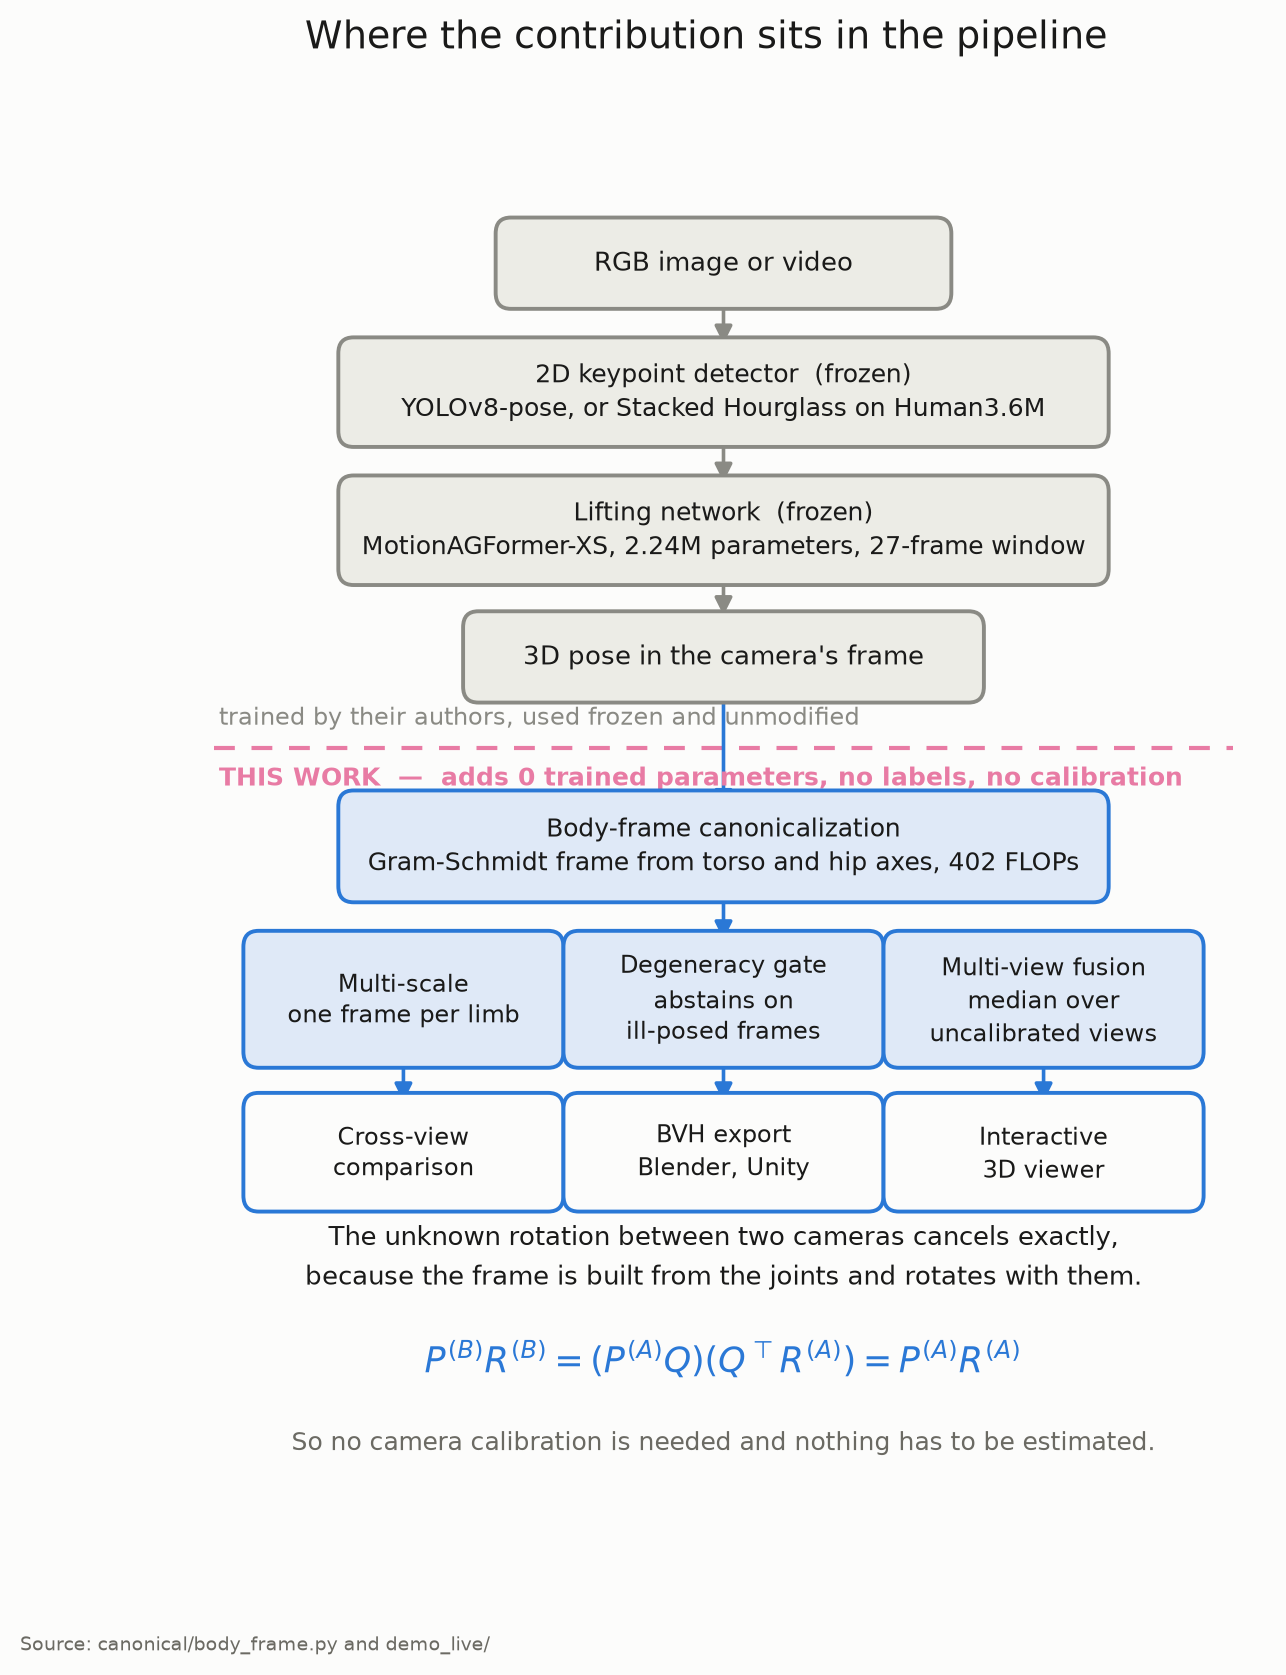
\includegraphics[width=0.86\textwidth]{images/fig_architecture.png}
\caption{The pipeline, with the contribution boundary marked. Everything above the dashed line is trained by its authors and used frozen and unmodified. Everything below it is contributed by this project and adds no trained parameters, consumes no labels and requires no camera calibration.}
\label{fig:arch}
\end{figure}

\begin{table}[h]
\centering
\caption{What each element of the pipeline requires}
\label{tab:freefrom}
\begin{tabular}{|l|c|c|}
\hline
\textbf{Element} & \textbf{Learned parameters} & \textbf{Labels} \\
\hline
YOLOv8-pose detector (frozen) & Trained by authors & Yes \\
\hline
MotionAGFormer-XS lifter (frozen) & Trained by authors & Yes \\
\hline
Canonicalization, multi-scale, fusion & \textbf{0} & None \\
\hline
Reliability score & \textbf{0} learned, 6 hand-set constants & None \\
\hline
Bone-length inconsistency & \textbf{0} & \textbf{None} \\
\hline
Component pruning (analysis only) & 0 & Uses ground truth \\
\hline
\end{tabular}
\end{table}

Three distinct claims follow. The framework adds zero learned parameters, which is what distinguishes it from 3DPCNet, itself estimator-agnostic but trained. The bone-length signal is additionally label-free. No component requires camera calibration. Conversely, the reliability score contains hand-set constants and is therefore not free of tuned parameters, and the component-pruning analysis of Section \ref{sec:relfails} consumes ground-truth error and is reported as analysis rather than as a deployable method.

The distinction is worth stating in operational terms, because the phrase invites an obvious objection: the pipeline plainly contains neural networks trained on labelled data, so in what sense is anything free. The answer is that the property claimed is a property of the deployment requirement, not of the pipeline's history. To apply this framework to a new estimator, a new camera or a new domain, a practitioner needs no training data, no labels, no calibration and no gradient step; they need a pose in the expected joint layout. To apply 3DPCNet to a new estimator, they need to train its rectification network. Both methods sit downstream of a trained estimator, and the difference between them lies entirely in what the user must supply.

This framing also determines what would falsify the claim. It is not falsified by the presence of a pretrained backbone, which is assumed. It is falsified if the method turns out to require tuning per dataset. We regard the Human3.6M results of Sections \ref{sec:h36mcv} and \ref{sec:h36mfuse} as the strongest available evidence on that point, since the constants were fixed on MPI-INF-3DHP and were not adjusted for the second dataset, on which the method was nevertheless applied to 180 unseen camera pairs.

\section{Body-Frame Canonicalization}

Let $P \in \mathbb{R}^{17\times 3}$ be a root-relative predicted pose in the H36M-17 joint convention. We construct a body-fixed orthonormal frame as

\begin{align}
\mathbf{y} &= \frac{P_{8} - P_{0}}{\lVert P_{8} - P_{0} \rVert}, \qquad
\mathbf{x}_{\text{raw}} = P_{1} - P_{4}, \\
\mathbf{z} &= \frac{\mathbf{x}_{\text{raw}} \times \mathbf{y}}{\lVert \mathbf{x}_{\text{raw}} \times \mathbf{y} \rVert},
\qquad
\mathbf{x} = \mathbf{y} \times \mathbf{z}, \\
R &= [\,\mathbf{x} \mid \mathbf{y} \mid \mathbf{z}\,], \qquad
P_{\text{can}} = P R .
\end{align}

Here $\mathbf{y}$ is the torso vertical axis and $\mathbf{x}_{\text{raw}}$ the hip axis, and the cross products complete a right-handed orthonormal basis by Gram-Schmidt orthonormalization. The construction is closed form, costs $O(17)$ operations per frame, and has no free parameters. Figure \ref{fig:framecon} shows it on a real predicted pose.

\begin{figure}[h]
\centering
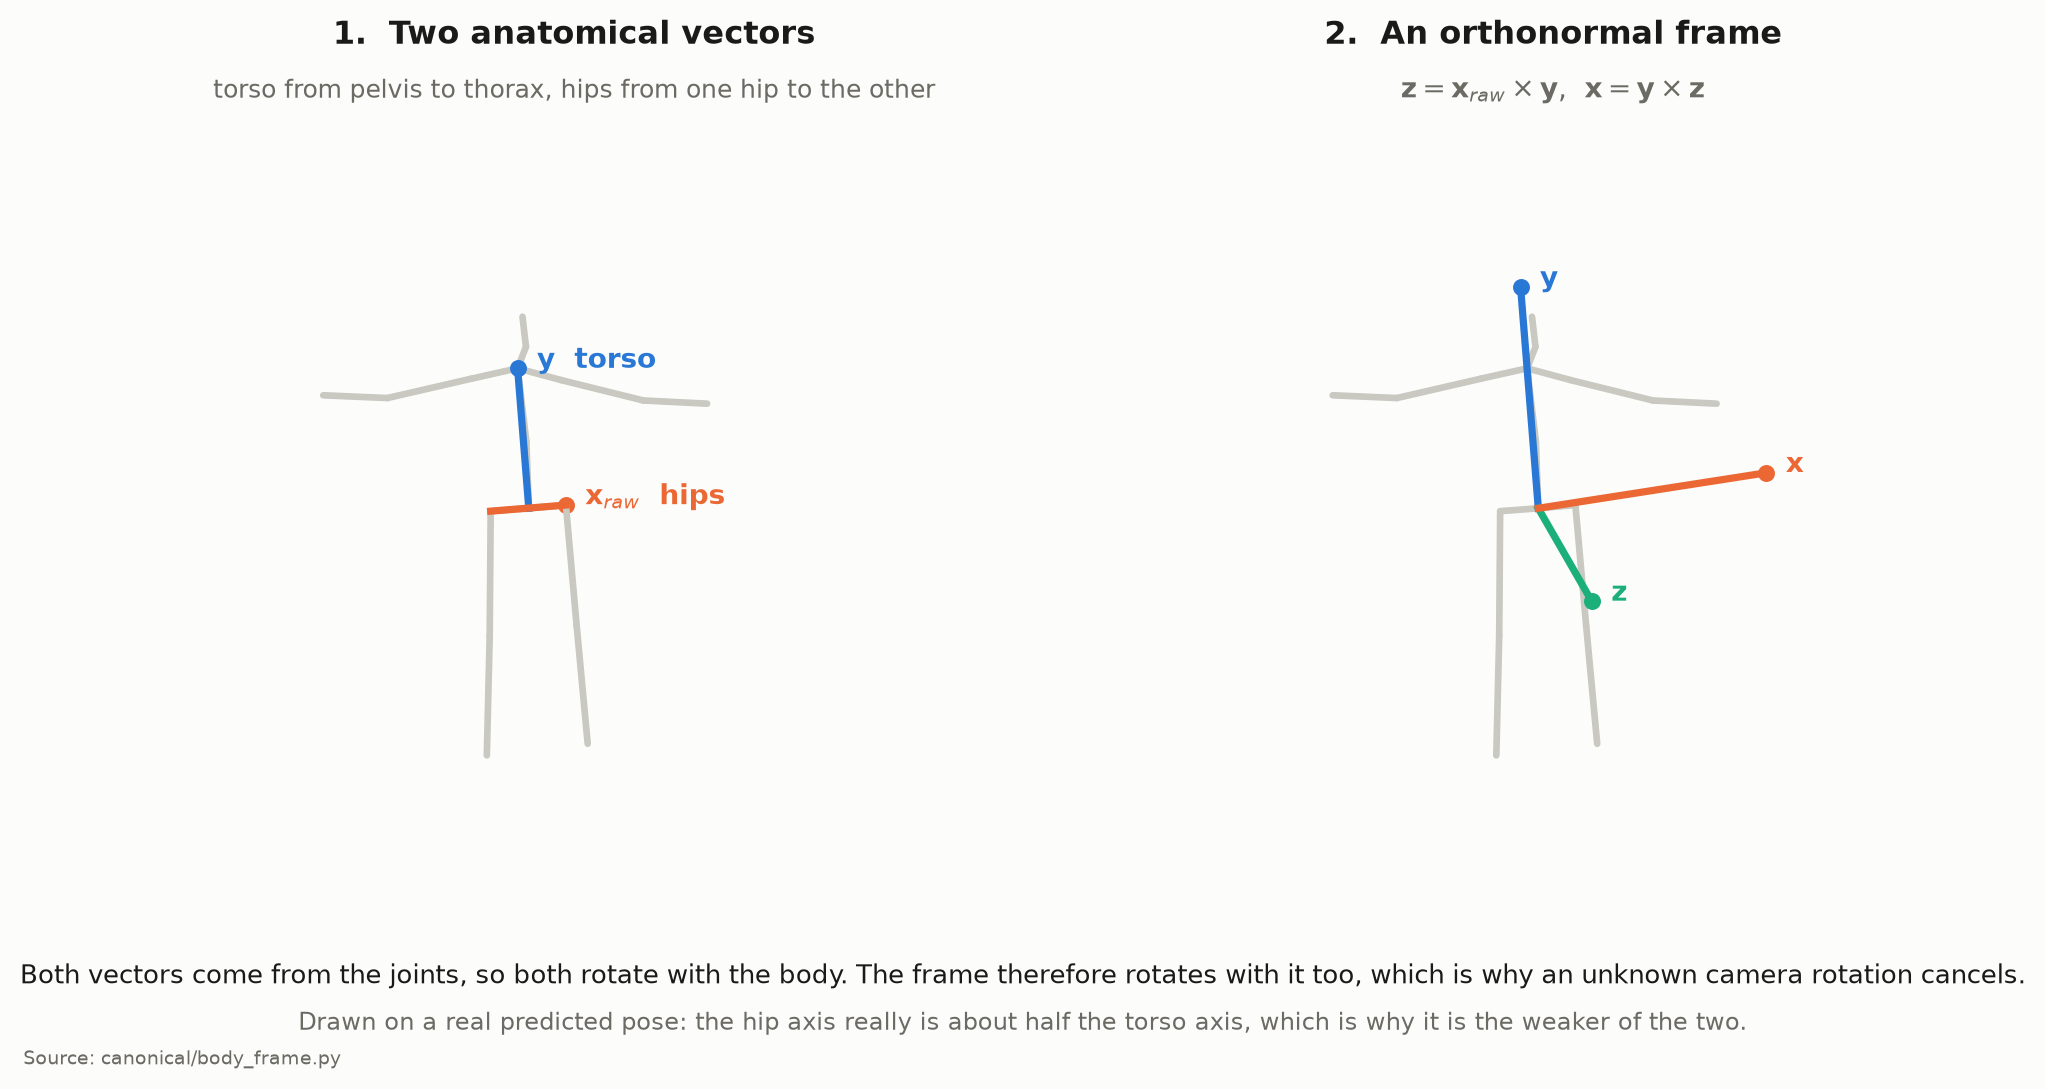
\includegraphics[width=\textwidth]{images/fig_frame_construction.png}
\caption{Constructing the body frame. Left: the two anatomical vectors the construction starts from. Right: the orthonormal triad Gram-Schmidt produces. Both source vectors are differences of predicted joints, so both rotate with the body, and the frame rotates with it.}
\label{fig:framecon}
\end{figure}

\subsection{Why This Construction Achieves View Invariance}

The property we require is that two cameras observing the same pose should produce the same canonical coordinates. Suppose cameras $A$ and $B$ observe one configuration, so that their root-relative predictions are related by an unknown rotation, $P^{(B)} = P^{(A)} Q$ for some $Q \in SO(3)$. Because the axes are constructed from the joint positions themselves, each axis rotates with the pose: the torso axis built from $P^{(B)}$ is the torso axis of $P^{(A)}$ rotated by $Q$, and likewise for the hip axis and for every vector derived from them by cross products. The frames therefore satisfy $R^{(B)} = Q^{\!\top} R^{(A)}$, and the canonical coordinates are
\begin{equation}
P^{(B)}_{\text{can}} = P^{(B)} R^{(B)} = \left(P^{(A)} Q\right)\left(Q^{\!\top} R^{(A)}\right) = P^{(A)} R^{(A)} = P^{(A)}_{\text{can}} .
\end{equation}
The unknown rotation cancels exactly, and it does so without ever being estimated. This is the reason no calibration is required: the method never needs to know $Q$, only that the frame co-rotates with the body.

The argument is exact for the idealized case in which both cameras yield the same pose up to rotation. In practice they do not, because each prediction carries its own error, and the frame is built from the erroneous joints rather than the true ones. The residual canonical distance we measure in Chapter 5 is precisely this term, which is why it does not fall to zero and why the per-frame Procrustes oracle, which aligns the two predictions optimally, is the appropriate floor rather than zero.

\subsection{Why Axis Length Governs Frame Stability}
\label{sec:axistheory}

The choice of axes is not arbitrary and the reason can be derived rather than asserted. Suppose a direction is estimated from two predicted joints separated by a distance $L$, each carrying independent isotropic position noise of standard deviation $\sigma$. The segment vector is a difference of two such positions, so its noise has variance $2\sigma^2$ per component. Only the component perpendicular to the segment rotates it, and that component has two degrees of freedom, giving $\mathbb{E}\lVert \boldsymbol{\epsilon}_{\perp}\rVert^2 = 4\sigma^2$. For small angles the induced angular error is therefore

\begin{equation}
\theta_{\mathrm{rms}} \;\approx\; \frac{2\sigma}{L} .
\label{eq:theta}
\end{equation}

Angular error is inversely proportional to the length of the segment the direction is read from. This is the statement Section \ref{sec:h36mms} arrives at empirically, and it also supplies the inverse-variance weight used in Section \ref{sec:multilandmark}: if variance scales as $L^{-2}$, the correct weight is $L^{2}$, which is derived rather than tuned.

Propagating equation \eqref{eq:theta} to the quantity we actually measure, a frame in error by $\theta$ displaces a joint lying at radius $r$ from the frame's origin by approximately $r\theta$. Two views canonicalized independently carry independent frame errors, so their disagreement adds in quadrature, and writing $\bar{r}$ for the mean joint radius and $d_0$ for the part of the disagreement that does not originate in the frame at all,

\begin{equation}
d^{2} \;\approx\; \Big(c\,\frac{\bar{r}}{L}\Big)^{2} + d_0^{2},
\qquad c = 2\sqrt{2}\,\sigma .
\label{eq:law}
\end{equation}

Equation \eqref{eq:law} is falsifiable, and Section \ref{sec:multilandmark} tests it.

\subsection{Sensitivity and the Choice of Axes}

The torso and hip axes are chosen because they are the longest and most reliably estimated directions available. Sensitivity of the frame to joint error scales inversely with the length of the defining vector, so a frame built from short segments would amplify noise, and the hip axis, at roughly half the torso axis, is the weaker of the two. Section \ref{sec:h36mms} confirms this experimentally for the per-limb frames.

We initially advanced the same argument to explain the SittingDown result of Section \ref{sec:h36mcv}, supposing that a seated pelvis is foreshortened and the hip axis correspondingly short. Measurement does not support that. Across the fifteen actions the hip axis of SittingDown is 285.3 mm, the second longest of any action, where WalkDog has the shortest at 268.4 mm and canonicalizes without difficulty. The angle between the hip and torso axes is 86.0 degrees for SittingDown, within the 83 to 88 degree range spanned by every other action, so the frame is not ill-conditioned either. We therefore withdraw the foreshortening explanation and give the supported one in Section \ref{sec:h36mcv}.

A further subtlety concerns sign. The hip axis direction depends on which hip is labelled left, and a prediction in which the two are exchanged produces a frame rotated by $\pi$ about the torso axis. For video we therefore carry the previous frame's forward axis and flip the current frame when the two disagree in sign, which enforces temporal consistency without imposing any prior on the pose itself.

\subsection{Computational Cost}

The title of this report claims the framework is lightweight, so we measure it rather than assert it. Table \ref{tab:cost} reports the cost of every component we add, against the frozen backbone it wraps.

\begin{table}[h]
\centering
\caption{Cost of the added framework, measured on real cached poses.}
\label{tab:cost}
{\fontsize{10}{12}\selectfont
\begin{tabular}{lrr}
\hline
\textbf{Component} & \textbf{Latency} & \textbf{Trainable parameters} \\
\hline
Canonicalization & 269 $\mu$s & 0 \\
Multi-scale, five frames & 1468 $\mu$s & 0 \\
Reliability score & 474 $\mu$s & 0 \\
Median fusion, four views & 215 $\mu$s & 0 \\
\hline
Frozen backbone, per frame & 11360 $\mu$s & 2\,240\,000 \\
\hline
\end{tabular}}
\end{table}

Two figures describe the overhead and they differ by four orders of magnitude, which is worth explaining rather than hiding. Counted in arithmetic, canonicalization is 402 floating-point operations per frame: a root subtraction, two differences, three normalizations, two cross products, a seventeen by three matrix product and an orthonormality check. Against roughly $7.6 \times 10^{7}$ operations for the backbone, estimated at two operations per parameter per token, that is 0.0005 percent. Measured in wall time it is 2.4 percent.

The gap is implementation, not algorithm. Our geometry is plain Python and NumPy over seventeen joints, where interpreter overhead dominates the arithmetic completely, while the backbone executes as compiled and vectorized tensor kernels. A batched or compiled implementation would approach the arithmetic ratio. We report the measured figure as the honest cost of the current code and the arithmetic figure as the cost of the method, and note that even the pessimistic figure leaves the framework at a fortieth of the estimator it wraps. Peak additional memory is 7560 bytes per call, which is the pose and a handful of three by three matrices.

Absolute latencies were measured while a second inference job occupied the same four-core machine and are therefore inflated; the ratio is the quantity to carry forward, and the arithmetic count is independent of load altogether.

\subsection{Degeneracy Handling}

Three configurations are detected and reported as invalid rather than silently returned: a torso axis shorter than five percent of the median bone length, a hip axis nearly parallel to the torso axis, so that the cross product is ill-conditioned, and a resulting matrix failing an orthonormality check. Invalid frames are excluded from every aggregate rather than replaced by a fallback, so that a reported mean is never diluted by frames on which the method declined to operate. On Human3.6M the construction is valid on every frame evaluated.

\section{Multi-Scale Per-Limb Frames}

The global frame removes orientation variation aligned with the torso, while limb orientations that differ from the torso remain. A raised arm, for example, is expressed in the same global frame as a lowered one, so its own orientation still varies with viewpoint through the residual error in the global frame estimate.

A separate frame is therefore constructed for each of five segments, namely the torso, left arm, right arm, left leg and right leg, by applying the same procedure to that segment's joints. Each segment's frame uses the segment's proximal-to-distal direction as its primary axis and the global torso axis as the secondary reference, which keeps the construction well defined even when a limb is straight and therefore provides only one independent direction of its own.

Two properties follow. Segments whose axes are near-degenerate fall back to the global frame, so the extension can never behave worse than the single-scale method on a degenerate limb. And because each segment is normalized separately, the representation discards the relative orientation between limbs, which is information a downstream task might need. This is a deliberate trade rather than a free improvement, and it is the same trade that makes the representation unsuitable for retrieval, as reported in the final section of Chapter 5.

\section{Analytic Reliability Score}

We compute six quantities from the predicted pose alone: axis conditioning, the angle between the torso and hip axes, bilateral symmetry of limb lengths, the fraction of anatomically abnormal bone ratios, the minimum detector keypoint confidence, and temporal stability of the body frame. Each is normalized to $[0,1]$ with hand-set constants, and they are combined by geometric mean,
\begin{equation}
r \;=\; \Big(\prod_{k=1}^{6} c_k\Big)^{1/6},
\end{equation}
so that any single catastrophic component drives the score toward zero rather than being masked by the others. Four hard geometric gates trigger abstention regardless of the combined score.

The design intent was that a geometrically implausible pose is unlikely to be an accurate one. Chapter 5 reports that this intent is not realized, and the reason is visible in the construction itself: every one of the six quantities is computed from a single frame's geometry, and a pose that is wrong purely in depth remains symmetric, correctly proportioned and well conditioned. The score is retained in the report because its failure is one of the project's substantive findings, and because the fusion experiments use it as a weighting scheme against which simpler alternatives are compared.

\section{Calibration-Free Multi-View Fusion}

Because canonicalization expresses every camera's prediction in the same body-fixed frame, predictions from $N$ uncalibrated cameras become directly comparable and may be combined without extrinsic parameters or correspondence search. This is the practical payoff of the cancellation shown above: triangulation requires the relative geometry of the cameras, whereas averaging in a shared body frame does not.

Given canonical poses $P^{(1)},\dots,P^{(N)}$ with reliabilities $r_i$, the weighted estimate is $\sum_i w_i P^{(i)}$ with $w_i = r_i / \sum_j r_j$, after resolving mirror ambiguity against the highest-weight view. We also evaluate the unweighted mean and the coordinate-wise median,
\begin{equation}
P_{\text{med}}[j,d] \;=\; \operatorname{median}_{i=1..N} P^{(i)}[j,d],
\end{equation}
which takes each coordinate of each joint independently and requires no weights at all.

The choice among these estimators is not cosmetic, and Section \ref{sec:h36mfuse} reports that it decides whether fusion helps or hurts. The reason is a difference in breakdown behaviour. A mean has a breakdown point of zero, so a single view whose frame is badly estimated shifts the result without limit, and its influence is $1/N$ of the total. A coordinate-wise median has a breakdown point approaching one half, so it is unaffected until nearly half the views fail. With $N=8$ a single failure contributes an eighth of a mean and is survivable; with $N=4$ it contributes a quarter and is not. This predicts that the advantage of the median over the mean should grow as the number of views falls, which is what we observe between the two datasets.

\section{Temporal Bone-Length Inconsistency}

A person's bones do not change length, so any temporal variation in predicted bone length is evidence of error, and monocular depth ambiguity produces exactly such variation through foreshortening. For each frame the sixteen bone lengths are divided by that frame's mean bone length, giving a scale-free ratio vector $\mathbf{b}_t$. The subject's skeleton is estimated as the median $\tilde{\mathbf{b}}$ over a reference window, using no labels, and the signal is

\begin{equation}
d_t \;=\; \frac{1}{16}\sum_{k=1}^{16}
          \frac{\lvert b_{t,k} - \tilde{b}_{k} \rvert}{\tilde{b}_{k}} .
\end{equation}

\section{Evaluation Protocol}
\label{sec:protocol}

Three properties of the protocol are essential to the validity of the results. Every reported frame is lifted from a true twenty-seven frame window of consecutive detections; an earlier protocol repeated a single frame twenty-seven times, and results obtained under it are not reported here. Only frames possessing a complete window are evaluated. The development pair, on which all tuning was performed, is identified explicitly in every table, and the remaining twenty-seven pairs together with the second subject are held out. Finally, no display transformation is applied in any quantitative path, and the prediction-versus-prediction metric is termed cross-view joint distance rather than MPJPE, which is reserved for comparisons against ground truth.

\subsection{Metrics}

Three distinct quantities appear in Chapter 5 and conflating them would be an error. Cross-view joint distance is the mean Euclidean distance between two root-relative predictions of the same instant from different cameras. It compares predictions to each other and never to ground truth, so it measures agreement rather than accuracy, and two views can agree perfectly while both are wrong.

Where ground truth is available we report a similarity-aligned distance, obtained by aligning the prediction to the ground truth with the optimal rotation, translation and isotropic scale in the sense of Umeyama [16] and then taking the mean per-joint distance. The alignment is used because the predictions and the annotations do not share a coordinate convention or a scale, and comparing them without it would measure the convention rather than the pose. We do not call this quantity MPJPE, which by convention denotes an unaligned root-relative comparison on the benchmark's own protocol. The one place we do report MPJPE is the pipeline verification in Section \ref{sec:h36m}, where reproducing the published figure is the entire purpose.

The per-frame Procrustes oracle aligns one prediction onto the other with the optimal rigid transform. It requires knowledge of the second view and is therefore not achievable by any single-view method; it appears as a floor against which the canonical distance is judged, since no rotation-based normalization can do better.

\subsection{Statistical Treatment}

Frames within a camera stream are not independent, since neighbouring windows overlap and neighbouring frames of a fifty hertz recording are near-duplicates. Treating them as independent would produce confidence intervals that are far too narrow. Where a quantity is reported with an interval, the interval comes from a cluster bootstrap of ten thousand draws that resamples whole camera streams on MPI-INF-3DHP and whole subject and action groups on Human3.6M, so the unit of resampling matches the unit of dependence. On Human3.6M this means thirty clusters rather than 180 camera pairs or 52900 frames, which is the honest count of how many independent observations the dataset actually supplies.

Reporting intervals changed two conclusions and we flag both rather than presenting only the outcome. The cross-view and multi-scale improvements are comfortably bounded away from zero. The fusion result is not uniformly so: the median's interval excludes zero while the unweighted mean's does not, which means the mean's apparent harm is a point estimate rather than a demonstrated effect. Section \ref{sec:h36mfuse} states the weaker claim that the interval supports. On Human3.6M we additionally subsample frames to five hertz before computing correlations, so that adjacent samples are not near-copies of one another. Reference skeletons are still estimated from every frame, since that estimate consumes no degrees of freedom from the comparison.

% ========================== CHAPTER 4 ================================
\chapter{DATASETS AND SYSTEM IMPLEMENTATION}

\section{MPI-INF-3DHP}

MPI-INF-3DHP is a markerless multi-camera capture dataset recorded in a green-screen studio with fourteen cameras, of which eight observe the subject from positions distributed around the room at two elevations. We use subjects S1 and S2, each recorded under a static condition in which the subject performs seated and standing motions with limited translation, and a dynamic condition involving walking, gesturing and larger displacement. The two conditions are treated as separate strata throughout, because a signal that behaves differently under translation is a signal whose scope must be stated.

Ground truth is supplied as \texttt{annot.mat}, containing camera-coordinate 3D annotations in a twenty-eight joint layout, together with a \texttt{camera.calibration} file giving intrinsics and extrinsics. We use the calibration only to verify that ground truth transported from two cameras into a common world frame agrees, which is a sanity check on our own reading of the data. No part of the method consumes calibration, and the framework has no access to it at inference.

The dataset is well suited to the central question because it provides many simultaneous views of the same instant. Twenty-nine camera pairs are formed, of which one is reserved as the development pair on which all tuning was performed, twenty-seven are held out on subject S1, and the remaining pair covers held-out subject S2.

\section{Human3.6M}

Human3.6M is the standard benchmark for monocular 3D pose estimation. Eleven subjects perform fifteen everyday actions while recorded by four hardware-synchronized cameras at fifty frames per second. Following the established protocol we train on nothing and evaluate on subjects S9 and S11, which the backbone did not see during its own training. Two cameras record at 1000 by 1002 pixels and two at 1000 by 1000, and the resolution is required to map normalized coordinates back to pixels.

The test split contains 566920 frames. We use the preprocessing distributed with the backbone, which slices the split into 20872 non-overlapping windows of twenty-seven frames. Where a video length is not divisible by twenty-seven the final window is resampled, so a small number of frames appear in two windows; these are averaged over their occurrence count, exactly as the official evaluation averages their errors.

Two properties make Human3.6M the right second dataset for this project. The four cameras are synchronized, so cross-view pairing needs no interpolation, and every one of the thirty subject and action groups in the test split has all four cameras with identical frame counts. Equally important, the dataset played no part in developing the method, so every camera pair formed from it is held out in a stronger sense than the MPI-INF-3DHP pairs, which share a dataset with the development pair.

\begin{table}[h]
\centering
\caption{The two evaluation datasets.}
\label{tab:datasets}
\begin{tabular}{lll}
\hline
\textbf{Property} & \textbf{MPI-INF-3DHP} & \textbf{Human3.6M} \\
\hline
Cameras used & 8 & 4 \\
Synchronized & yes & yes \\
Test subjects & S1, S2 & S9, S11 \\
Conditions & static, dynamic & 15 actions \\
2D front end & YOLOv8-pose & Stacked Hourglass \\
Backbone domain & out-of-domain & in-domain \\
Camera pairs evaluated & 29 & 180 \\
Pairs held out & 27 & 180 \\
Median aligned error & 202.1 mm & 32.6 mm \\
\hline
\end{tabular}
\end{table}

The final row of Table \ref{tab:datasets} deserves emphasis, because it explains several results in the next chapter. The backbone is roughly six times more accurate on Human3.6M than on MPI-INF-3DHP. It was trained on Human3.6M subjects and is evaluated there on held-out subjects of the same capture setup, whereas MPI-INF-3DHP presents a different studio, a different 2D detector and a joint layout that must be mapped. The two datasets therefore probe different regimes rather than merely repeating one another.

\section{Joint Conventions and the Mappings Between Them}

Three joint layouts appear in this project and confusing them is a silent source of error, so we state them explicitly. The backbone consumes and produces the seventeen-joint Human3.6M layout, in which joint 0 is the pelvis root, joints 1 to 3 and 4 to 6 are the right and left legs, joints 7 to 10 run up the spine to the head, and joints 11 to 16 are the two arms. The 2D detector used on MPI-INF-3DHP emits the seventeen-joint COCO layout, which has facial keypoints instead of a spine and no pelvis, so the pelvis and thorax are synthesized by interpolation before lifting. Ground truth in MPI-INF-3DHP uses a twenty-eight joint layout from which seventeen are selected.

The torso correspondences are approximate in both directions, because COCO has no spine joint and the twenty-eight joint layout places its spine points differently from Human3.6M. Limbs and hips correspond exactly. We report this rather than suppress it, since it inflates the ground-truth error on MPI-INF-3DHP by an amount we do not attempt to separate, and it is one reason the two datasets are not directly comparable in absolute millimetres.

\section{Implemented System}

The framework is implemented in Python on PyTorch as a post-processing layer, and it is deliberately separable from the estimator it wraps. The canonicalization module consumes a seventeen by three array and returns a canonical pose, a rotation matrix and a validity flag, so any estimator producing that layout can be substituted without modification. The evaluation modules are organized one per experiment, each writing a JSON artifact under a common directory, and each runnable independently.

Three engineering decisions carry scientific weight. First, the lifting path used by the evaluation is the same code as the demonstration application, extracted into a shared module so that reported numbers and demonstrated behaviour cannot diverge. Second, predictions are cached per camera, so an analysis can be re-run without re-running inference, which is what made the Human3.6M experiments of the next chapter affordable. Third, every headline number is recomputed from its artifact by an automated audit, described in Section \ref{sec:protocol}, which fails if any number drifts.

An interactive demonstration built with Gradio accepts an uploaded image or video, runs detection and lifting, and displays the raw and canonical skeletons side by side together with the reliability score and its six components. It also exports a canonicalized sequence as a BVH motion-capture file, which animation software imports directly; that format stores joint rotations relative to each parent and contains no camera, so it is the natural consumer of a body-fixed frame. The demonstration exists to make failure modes visible rather than to add a result, and it was the route by which several were noticed, including a rendering fault that drew canonical skeletons on their side in the video path.

Figure \ref{fig:qual} shows the system on frames of that demonstration footage, which belongs to neither evaluation dataset. The third row is included because it fails: a subject bent sharply forward foreshortens the torso, and the reconstruction is visibly poorer. A qualitative figure showing only successes would misrepresent a method whose weakest measured action is a seated one.

\begin{figure}[h]
\centering
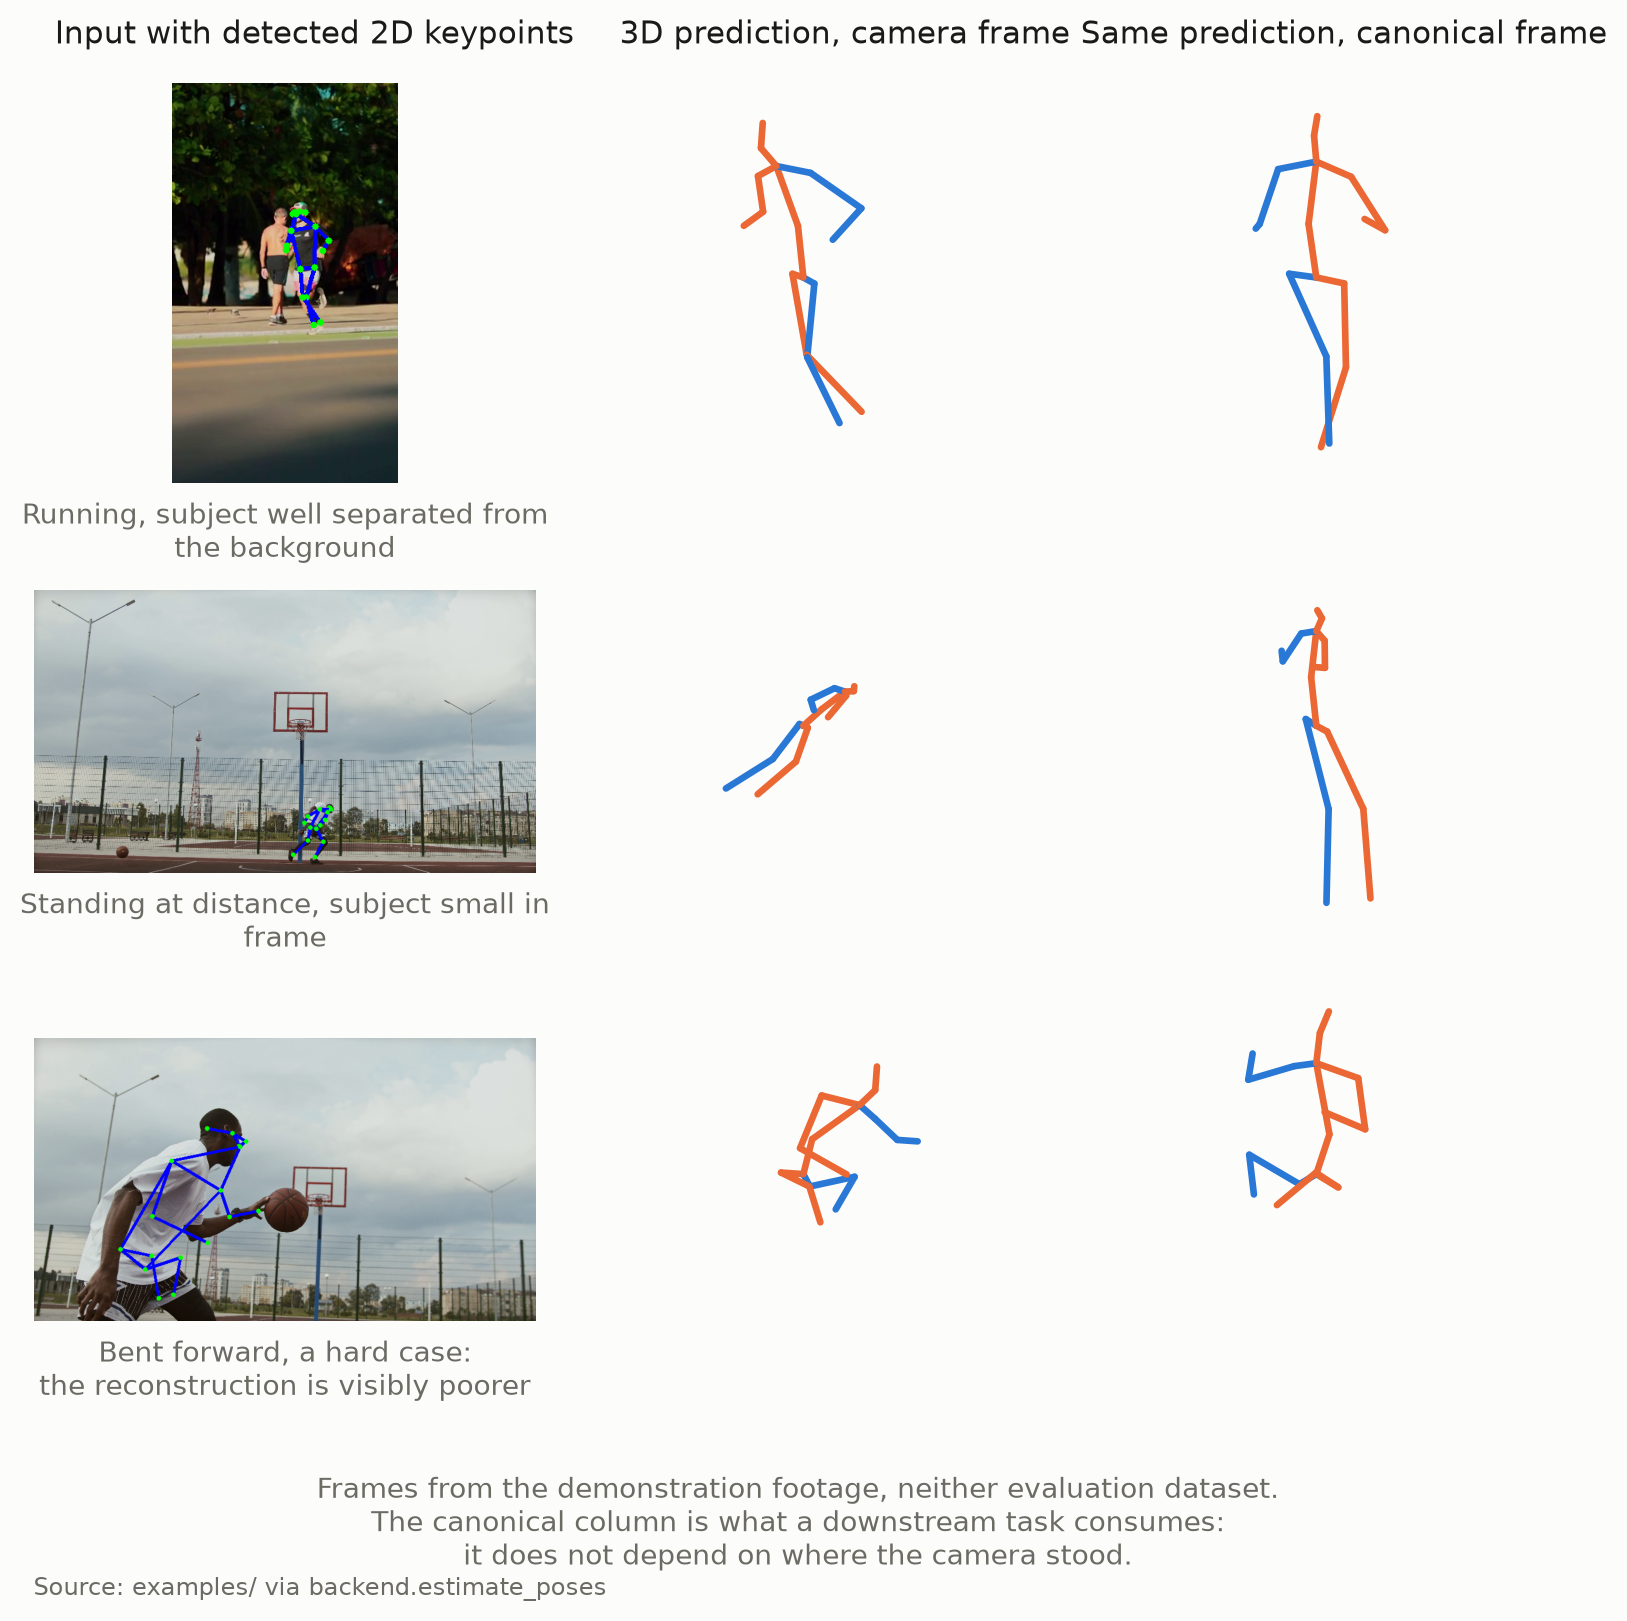
\includegraphics[width=\textwidth]{images/fig_qualitative.png}
\caption{The pipeline on uncontrolled footage. Left: input with detected 2D keypoints. Middle: the 3D prediction in the camera's frame. Right: the same prediction in the body-fixed frame, which is what a downstream task consumes.}
\label{fig:qual}
\end{figure}

\section{Reproducibility Infrastructure}

The reporting practice adopted here is a response to the fact that several early claims in this project did not survive scrutiny. Three mechanisms are used. The automated audit re-derives sixty-five headline claims from stored artifacts and fails on any drift, so a number cannot silently rot after a re-run. A unit test suite of ninety tests covers the geometric core, the corruption operators, the fusion arithmetic and the aggregation logic of the Human3.6M experiments, using stub models so that it runs without weights or data. Finally, the pass criterion for the test-time augmentation experiment was written down and committed to version control before that experiment was run, so its failure cannot be attributed to a criterion chosen afterwards.

The appendix tables are generated from the artifacts by a script rather than typed, which closes the last gap between what the artifacts contain and what the report claims.

% ========================== CHAPTER 5 ================================
\chapter{EXPERIMENTAL RESULTS AND OBSERVATIONS}

\section{Summary of Findings}

This chapter reports both confirmations and failures, and the failures are numerous enough that the reader deserves the outcome before the argument. Table \ref{tab:summary} states every claim tested and its verdict. Three components hold on both datasets, one was refined by testing, and two were withdrawn.

\begin{table}[h]
\centering
\caption{Every claim tested in this chapter, and its verdict on each dataset.}
\label{tab:summary}
{\fontsize{10}{12}\selectfont
\begin{tabular}{p{4.6cm}p{3.1cm}p{3.1cm}l}
\hline
\textbf{Claim} & \textbf{MPI-INF-3DHP} & \textbf{Human3.6M} & \textbf{Verdict} \\
\hline
Canonicalization improves cross-view comparability
 & $+32.4\%$, 27 held-out pairs
 & $+74.1\%$, 180 held-out pairs, 179 improve
 & Holds \\
\hline
Multi-scale per-limb frames improve on the global frame
 & 29 of 29 pairs
 & $+25.6\%$, and $+55.1\%$ once every frame uses its own long axis
 & Holds \\
\hline
The shared frame enables calibration-free fusion
 & Improves in all four conditions
 & Median $+8.4\%$; an unweighted mean is not reliably better than one view
 & Holds, refined \\
\hline
The reliability score predicts accuracy
 & Fails on five independent tests
 & Fails again; weighting by it is indistinguishable from using one camera
 & Withdrawn \\
\hline
Bone-length inconsistency predicts error
 & $\rho = +0.492$
 & $\rho = +0.098$, all five criteria fail
 & Withdrawn \\
\hline
Canonicalization aids cross-view retrieval
 & Recall falls
 & Not tested
 & Withdrawn \\
\hline
\end{tabular}}
\end{table}

The positive results concern comparability rather than accuracy, which is the property this project set out to provide, and the distinction is maintained throughout. The one exception is fusion, which combines several views into a single estimate and therefore does reduce error against ground truth.

\section{Experimental Setup}

We evaluate the framework on the MPI-INF-3DHP dataset [10]. Eight synchronized cameras of subject S1 sequence 1 give twenty-eight camera pairs, and a pair from subject S2 provides a held-out subject. We extracted frames from the dataset's own video files, and verified frame indices against the annotation file by projecting the 2D ground truth onto the extracted images. To test conditions under which viewpoint quality varies within a sequence, we selected a dynamic window containing 138 degrees of net body rotation using a ground-truth motion scan. The frozen lifting network is MotionAGFormer-XS, whose Human3.6M reproduction matches the published figures at 45.149 mm against 45.1 mm.

Ground-truth error is computed after a similarity alignment of rotation, translation and scale, and is not termed MPJPE because the alignment protocol differs from the standard benchmark definitions. All reported numbers are recomputed from stored artifacts by an automated audit covering forty claims.

\section{Cross-View Consistency}
\label{sec:crossview}

\begin{table}[h]
\centering
\caption{Cross-view joint distance improvement under canonicalization}
\label{tab:crossview}
\begin{tabular}{|l|c|c|}
\hline
\textbf{Scope} & \textbf{Pairs} & \textbf{Improvement} \\
\hline
Development pair (S1, cameras 0--1) & 1 & +20.5\% \\
\hline
Held-out pairs (S1) & 27 & \textbf{+32.4\%} \\
\hline
Held-out subject (S2) & 1 & +13.4\% \\
\hline
\end{tabular}
\end{table}

Table \ref{tab:crossview} summarizes the result and Figure \ref{fig:pairs} shows it pair by pair. The mean improvement on held-out pairs exceeds that on the development pair, which indicates that the result is not an artifact of tuning. Two pairs regress slightly, and both are near-aligned camera configurations whose raw cross-view distance is already small, leaving little orientation variation to remove. Figure \ref{fig:oracle} places these distances against a per-pair Procrustes oracle, which requires both poses jointly and therefore bounds what any rotation-based method can achieve.

\begin{figure}[h]
\centering
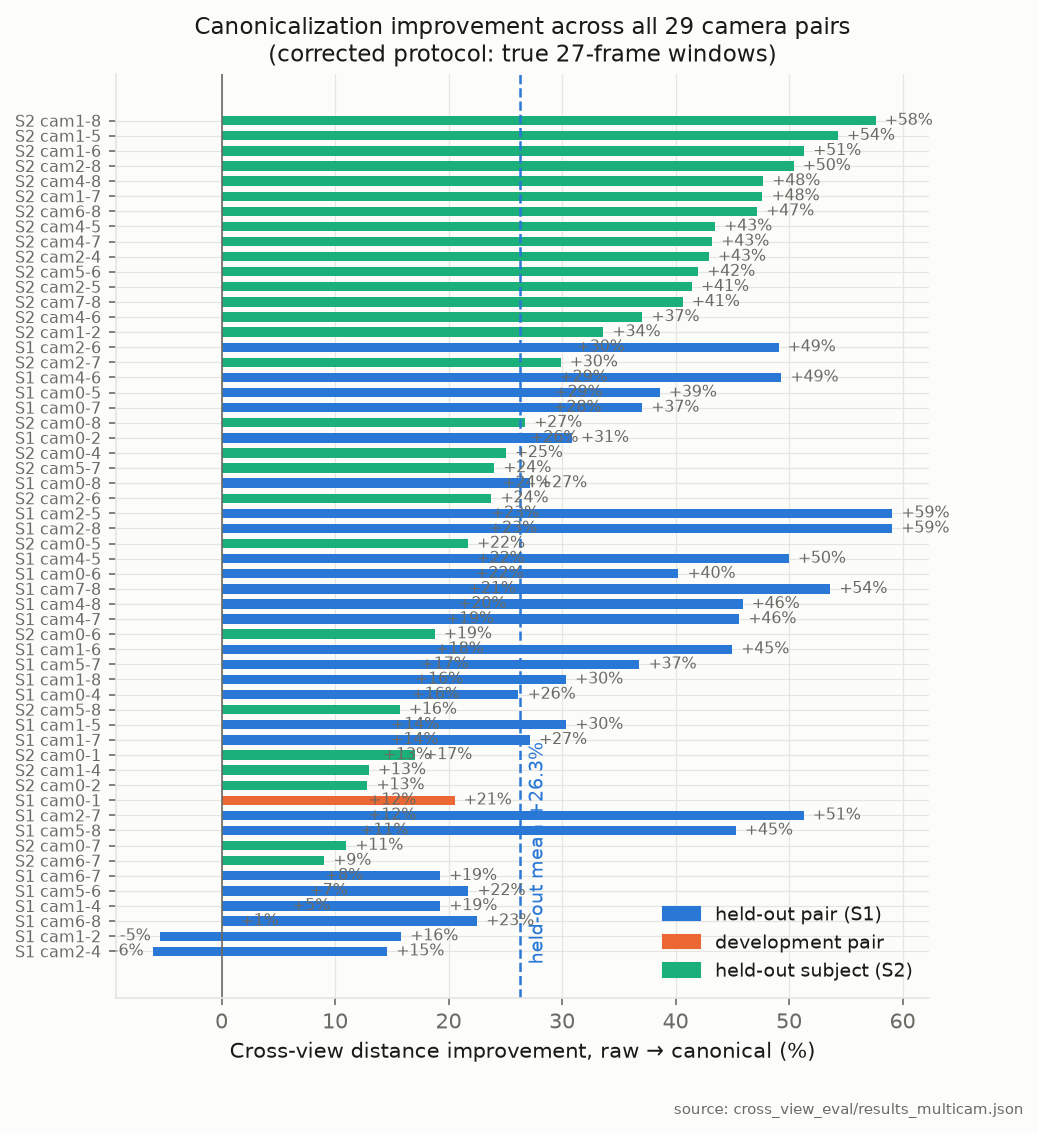
\includegraphics[width=0.75\textwidth]{images/fig_29pairs.png}
\caption{Improvement across all twenty-nine camera pairs}
\label{fig:pairs}
\end{figure}

\begin{figure}[h]
\centering
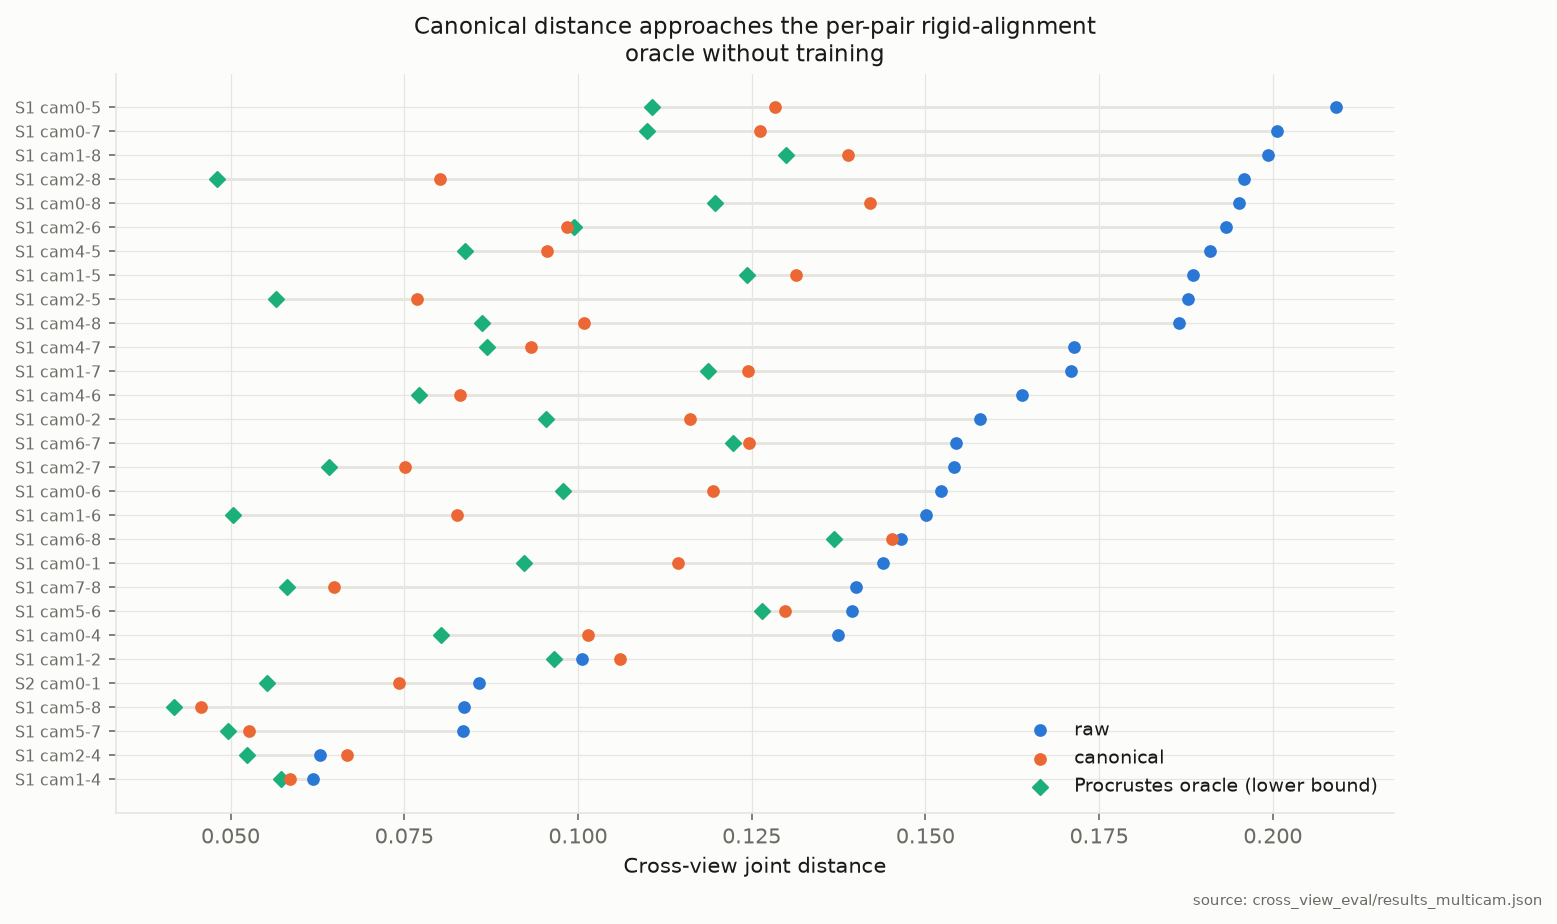
\includegraphics[width=0.75\textwidth]{images/fig_oracle.png}
\caption{Raw, canonical and Procrustes oracle distances per pair}
\label{fig:oracle}
\end{figure}

\newpage

\section{Ground-Truth Anchoring}

Cross-view consistency compares two predictions to each other and is in principle insensitive to errors shared by both views, so we anchor it against ground truth. World-transformed ground truth from different cameras agrees to 0.00 mm, which confirms that the reference frame is view-independent. We find that canonical cross-view distance correlates with true prediction error at a Spearman coefficient of $+0.601$ over 1566 frames, against $+0.188$ for the raw distance. This suggests that canonicalization makes cross-view consistency a substantially stronger proxy for actual error.

\section{Reliability Under Controlled Degradation}

We applied five physically motivated corruptions at graduated severities over a sweep of 2240 records. Reliability tracks induced error at a Spearman coefficient of $-0.813$, joint dropout produces abstention in 100 percent of cases, and clean frames produce abstention in none. Identity-severity controls reproduced the clean baseline exactly. Figure \ref{fig:degradation} shows the relationship for each operator.

\begin{figure}[h]
\centering
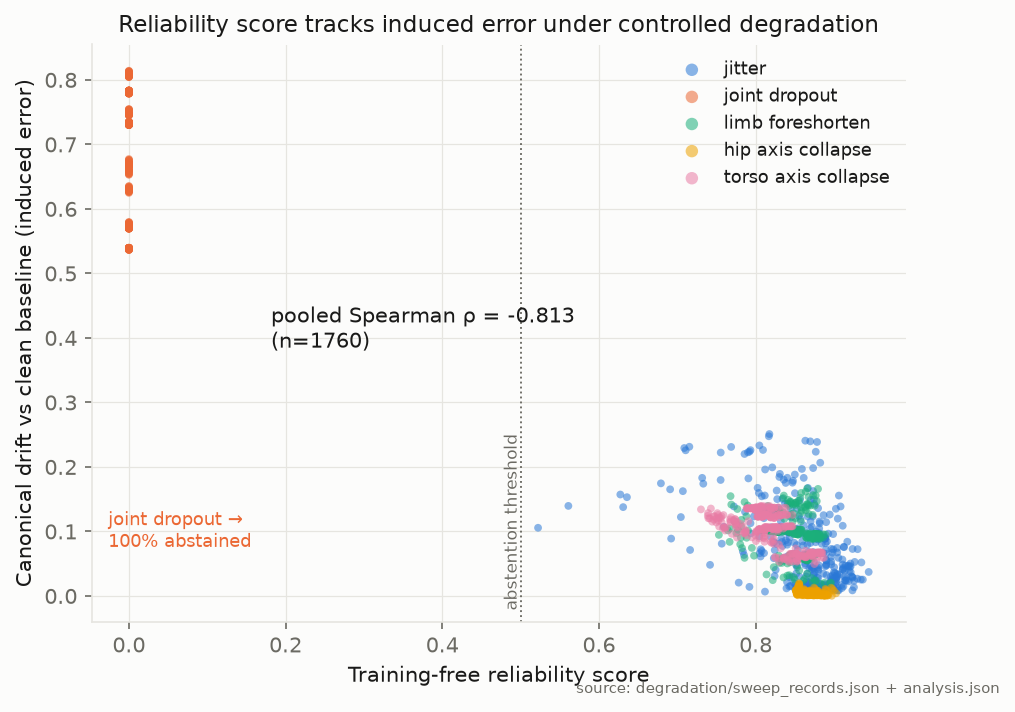
\includegraphics[width=0.72\textwidth]{images/fig_degradation.png}
\caption{Reliability against induced error for five corruption operators}
\label{fig:degradation}
\end{figure}

\section{Multi-Scale Canonicalization}

Per-limb frames improve every one of the twenty-nine pairs, by 37.1 percent on the development pair and by 36.4 percent on average over held-out pairs. The improvement is not an artifact of reduced degrees of freedom, since the multi-scale distance retains its correlation with ground-truth error at $+0.610$ against $+0.601$ for the global frame. Figure \ref{fig:multiscale} shows the per-pair gain.

\begin{figure}[h]
\centering
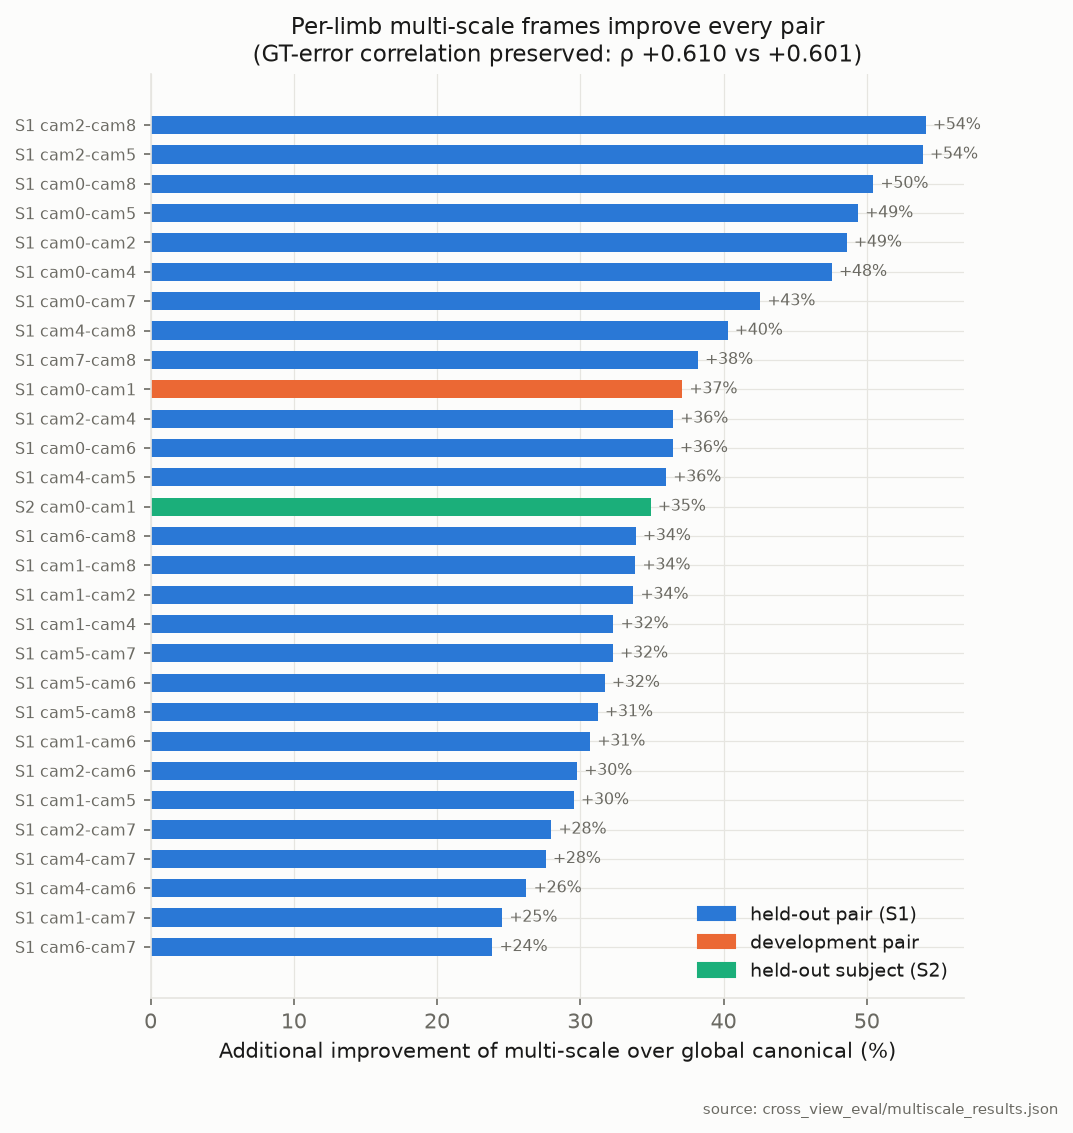
\includegraphics[width=0.7\textwidth]{images/fig_multiscale.png}
\caption{Additional improvement of multi-scale over global canonicalization}
\label{fig:multiscale}
\end{figure}

\newpage

\section{Multi-View Fusion and a Negative Result on Selection}

Fusion improves on an arbitrary single view in all four conditions, by 23.7 and 10.6 percent on subject S1 under static and dynamic motion and by 10.2 and 8.2 percent on subject S2. Because averaging does not require knowing which view is best, the result is robust. Figure \ref{fig:fusion} shows how the gain scales with the number of available cameras while the single-view baseline stays flat.

Selection, by contrast, does not survive scrutiny. We initially measured a 33.8 percent gain from selecting the most reliable view, but we find this to be an artifact: on static footage the score selects the same camera in every frame, and the gain arises from that constant choice combined with a large spread of per-view error. On dynamic sequences the selected view's true-error rank is 4.78 of 8 on subject S1 against a chance expectation of 4.5, and 3.67 on subject S2, straddling chance in opposite directions. We therefore withdraw the claim.

\begin{figure}[h]
\centering
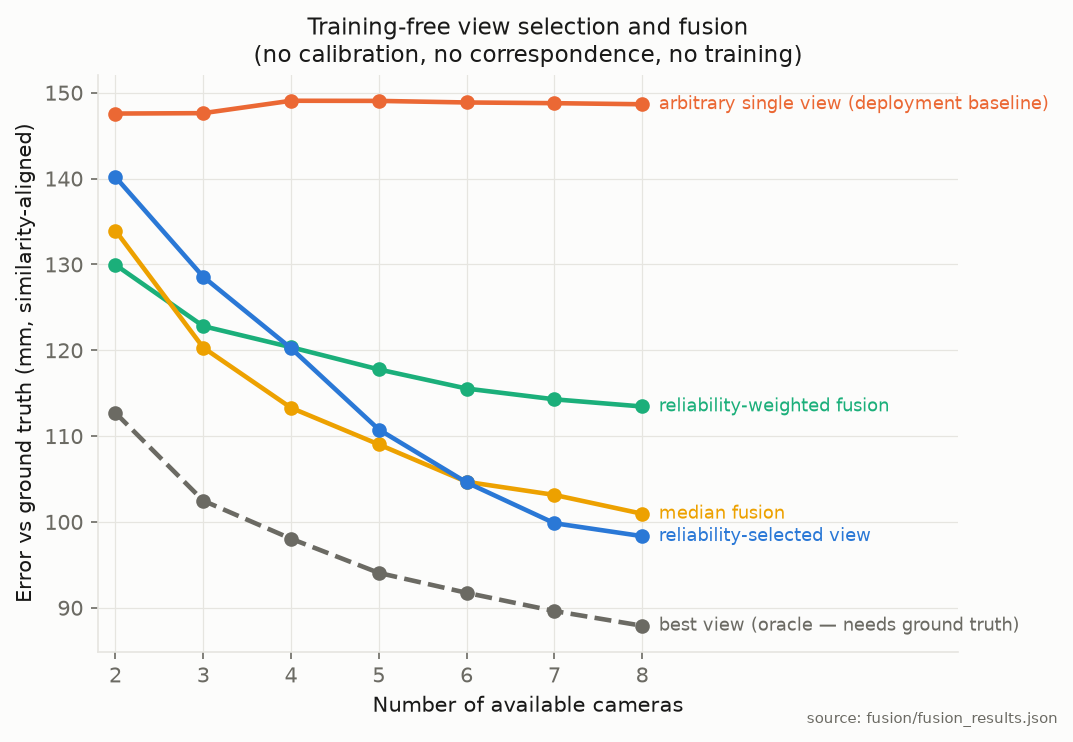
\includegraphics[width=0.75\textwidth]{images/fig_fusion.png}
\caption{Error against number of available cameras for each strategy}
\label{fig:fusion}
\end{figure}

\section{Why the Reliability Score Fails and What Succeeds}
\label{sec:relfails}

We conducted five independent experiments that falsify the reliability score as a predictor of accuracy. Within a frame, its correlation with per-view error across simultaneous cameras is approximately zero. View selection straddles chance, as described above. Its sign inverts across backbones, at $-0.707$ on MotionBERT against $+0.375$ on a multilayer perceptron baseline. Reliability-weighted fusion of heterogeneous models is worse than an unweighted mean. Finally, we pre-registered a pass criterion for test-time augmentation dispersion and committed it to version control before running that experiment; the result failed all three criteria, with a coefficient of $+0.100$, inconsistent signs across strata, and a bootstrap interval spanning zero.

We attribute these results to a single cause. The score measures within-frame geometric plausibility, which a coherent depth error leaves intact, since a pose can be symmetric, correctly proportioned and well conditioned while being wrong in depth. The score therefore detects corruption, which destroys plausibility, but not the depth ambiguity that dominates monocular estimation. The failure of test-time augmentation sharpens this point, because it indicates that the model agrees with itself while being wrong, so self-consistency carries little error information.

A constraint enforced by the world rather than by the model does carry that information. We find that temporal bone-length inconsistency predicts error at a Spearman coefficient of $+0.492$ over 2460 frames, with the same sign in all four strata. It is not a proxy for detector confidence, since the partial correlation controlling for confidence is $+0.481$; it is not an artifact of scale, since the scale-free formulation scores $+0.492$ against $+0.367$ for scale alone; and it is not transductive, since a causal reference window disjoint from the scored frames gives $+0.473$ and a skeleton estimated from a different camera gives $+0.440$. A cluster bootstrap over cameras places the improvement over the incumbent score in the interval $[+0.108, +0.515]$. Every figure in this paragraph describes MPI-INF-3DHP alone. Section \ref{sec:h36m} tests whether they survive on a second dataset, and reports that they do not.

The signal is nevertheless frame-level rather than joint-level. Assigning each joint the deviation of its adjacent bones yields chance-level ranking within a frame, so it supports triage of whole predictions but not spatial localization of error.

Component analysis further shows that the incumbent score's weakness lies in its combination rule rather than in its parts. Four of the six components individually predict error roughly twice as well as their geometric mean. Selecting components on subject S1 and scoring on held-out subject S2 raises the held-out coefficient from $-0.162$ to $-0.357$, and combining the pruned composite with the bone-length signal reaches $+0.395$. This analysis uses ground-truth error for selection and is therefore reported as diagnosis rather than as a deployable method.

\section{Replication on Human3.6M and Retraction of the Bone-Length Claim}
\label{sec:h36m}

The result of the preceding section rests on one dataset, one two-dimensional front end and one recording setup, so we repeat the experiment on Human3.6M. Three conditions change together. The dataset changes from MPI-INF-3DHP to Human3.6M, the two-dimensional front end changes from YOLOv8 to Stacked Hourglass, and the operating regime changes from out-of-domain to in-domain, because the backbone was trained on subjects S1 to S8 of Human3.6M and we evaluate on the held-out subjects S9 and S11. We follow the official evaluation path of the backbone exactly, and we verify that path by reproducing its published accuracy. Our pipeline yields 45.149 mm, which matches to three decimal places the figure obtained by running the evaluation script of the backbone itself, against 45.1 mm reported in its paper. The verification is worth stating precisely, because a failed replication is informative only if the apparatus is not what failed. We then apply the five criteria of Section \ref{sec:relfails}, with the clustering unit changed from camera to video and the strata changed from subject and condition to subject and camera.

The signal does not replicate. Over 52900 frames drawn from 228 videos the coefficient is $+0.098$, against $+0.492$ on MPI-INF-3DHP, and all five criteria fail. The sign is inconsistent across the eight subject and camera strata, which range from $-0.080$ to $+0.385$. The partial correlation controlling for detector confidence falls to $+0.014$, so the small remaining association is largely a restatement of confidence. A cluster bootstrap over videos places the difference from the incumbent reliability score in the interval $[-0.163, -0.063]$, which excludes zero in the direction that favours the incumbent. We note that the pre-registered wording of this criterion was two-sided and is therefore satisfied by this interval; we report the directional reading instead, because an interval lying below zero contradicts rather than supports the hypothesis.

A second observation was not anticipated. The reliability score replicates where the new signal does not, at $-0.212$ on Human3.6M against $-0.192$ on MPI-INF-3DHP. The component that failed five tests transfers across datasets, while the component that passed them does not.

Two explanations are available for the failure, and they can be separated. The first is that the original correlation was spurious. The second is that Human3.6M presents little for the signal to read, because the backbone is accurate in-domain. We test the second explanation by comparing the coefficient of each video against the mean error of that video, a between-video comparison that avoids the range restriction which a within-video split on error would introduce. The relationship is weak at $+0.152$ over 228 videos. The hardest third of videos gives a mean coefficient of $+0.156$ at 45.5 mm, against $+0.136$ at 28.3 mm for the easiest third. Difficulty within Human3.6M therefore does not recover the signal.

The two datasets nevertheless occupy different regimes, and the separation is large. The median similarity-aligned error is 202.1 mm on MPI-INF-3DHP against 32.6 mm on Human3.6M, and the median bone deviation is 0.082 against 0.034. We therefore read the signal as an indicator of gross skeletal deformation rather than of pose error in general. A backbone driven far outside its training distribution returns skeletons whose bone lengths visibly fluctuate, and the signal tracks that fluctuation. A backbone operating in-domain returns skeletons that are nearly rigid and still wrong in depth, and the signal has nothing left to measure.

\begin{figure}[h]
\centering
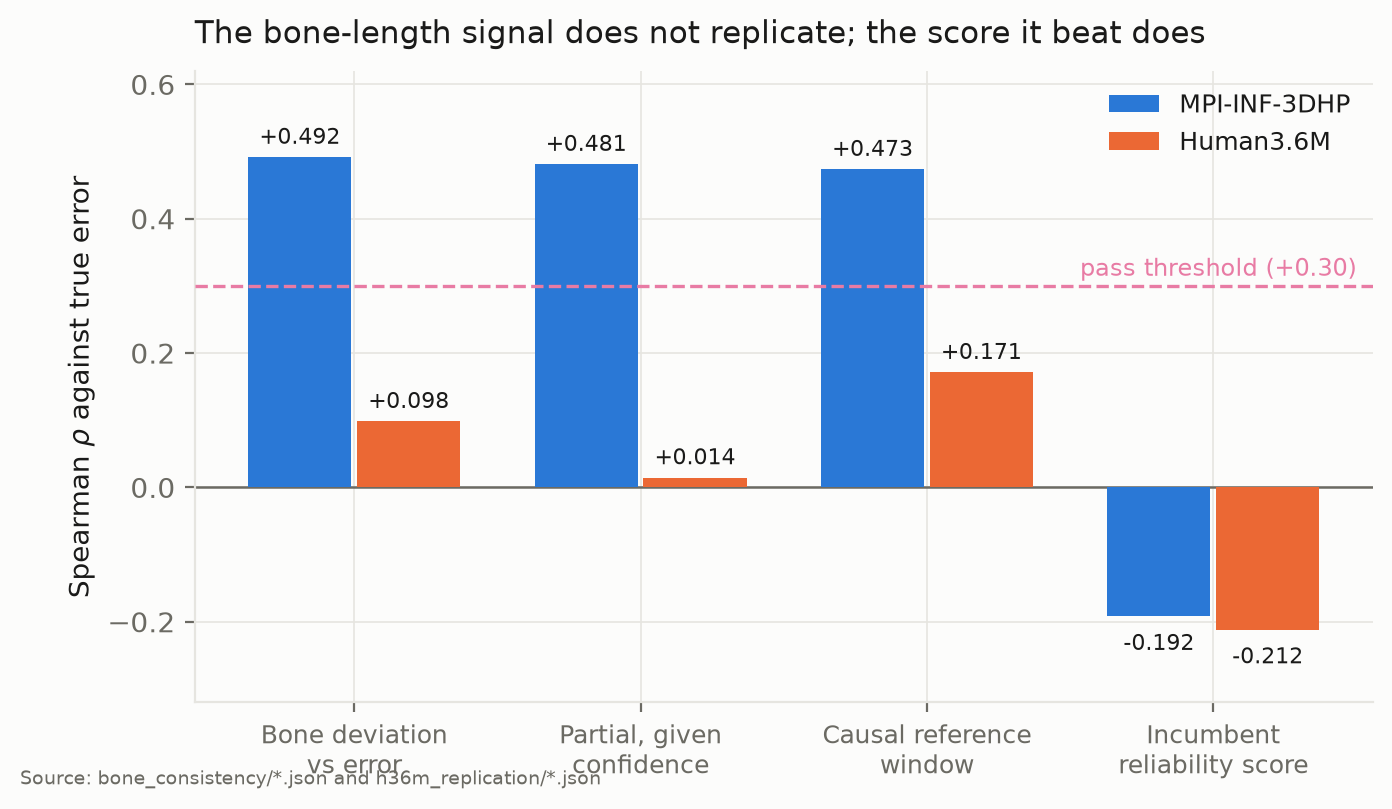
\includegraphics[width=0.95\textwidth]{images/fig_h36m_bone.png}
\caption{The bone-length signal on both datasets. Every measure that passed on MPI-INF-3DHP falls below the threshold on Human3.6M, while the reliability score it was introduced to replace transfers unchanged.}
\label{fig:h36mbone}
\end{figure}

This is the mechanism of Section \ref{sec:relfails} extended along the time axis. Within-frame plausibility is invariant to a coherent depth error, and bone-length consistency across frames is invariant to a temporally coherent depth error. We therefore retract the general claim and retain the narrower one that the evidence supports. Temporal bone-length inconsistency detects domain shift severe enough to deform the predicted skeleton, and it does not rank residual depth error in the regime where a backbone is already accurate.

\section{Cross-View Canonicalization on Human3.6M}
\label{sec:h36mcv}

The failure in Section \ref{sec:h36m} raised a sharper question about everything else in this chapter. If one result from MPI-INF-3DHP does not transfer, the central claim deserves the same test rather than our confidence. We therefore repeat the cross-view experiment on Human3.6M using the predictions already computed for the replication above.

Human3.6M suits the test well. Its four cameras are hardware synchronized, and every one of the thirty subject and action groups in the test split has all four cameras with identical frame counts, so pairing requires no interpolation and no timestamp matching. Four cameras yield six pairs per group and therefore 180 camera pairs, against the twenty-nine evaluated on MPI-INF-3DHP. Human3.6M played no part in developing the method, so unlike the earlier protocol there is no development pair to exclude: all 180 pairs are held out, as are both subjects.

The central claim replicates, and it replicates more strongly than it did on the dataset where the method was designed. Table \ref{tab:h36mcv} reports the result. Canonicalization reduces mean cross-view joint distance from 320.4 mm to 75.3 mm, an improvement of 74.1 percent, against 32.4 percent on MPI-INF-3DHP. It improves 179 of 180 pairs. A cluster bootstrap that resamples whole subject and action groups, rather than individual pairs, places the improvement in the interval $[+69.8, +77.2]$ percent. The clustering matters here: the six pairs of a group are formed from the same four camera streams of the same motion, so resampling pairs individually would treat 180 dependent observations as independent and return an interval that is too narrow. The interval excludes the 32.4 percent obtained on MPI-INF-3DHP by a wide margin, so the difference between the two datasets is not attributable to sampling. The per-frame Procrustes oracle reaches 51.3 mm, so canonicalization closes 90.5 percent of the gap between an arbitrary pair of viewpoints and the best a rotation can achieve. The body frame is well conditioned on every frame evaluated, giving a validity rate of 100 percent.

That comparison invites an obvious question, which we answer here rather than leave standing: if the oracle is better, why not simply use it. The oracle aligns two poses to each other, so it requires both of them at once, and what it returns is a relative alignment rather than a representation. It cannot canonicalize a single pose, because there is nothing to align that pose to; it cannot run before a comparison exists, so it cannot be used to index, store or stream; and with $N$ cameras it must be recomputed for each of the $N(N-1)/2$ pairs, whereas a body frame is computed once per pose and every pair is then comparable by construction. The oracle is included as a floor on what any rotation can achieve, not as a competing method. The relevant claim is that a construction which sees one pose at a time recovers most of what a construction that sees both can do.

\begin{table}[h]
\centering
\caption{Cross-view canonicalization on Human3.6M, 180 held-out camera pairs.}
\label{tab:h36mcv}
\begin{tabular}{lrr}
\hline
\textbf{Quantity} & \textbf{Human3.6M} & \textbf{MPI-INF-3DHP} \\
\hline
Camera pairs & 180 & 29 \\
Pairs held out & 180 & 27 \\
Raw cross-view distance & 320.4 mm & --- \\
Canonical cross-view distance & 75.3 mm & --- \\
Procrustes oracle & 51.3 mm & --- \\
Mean improvement & +74.1\% & +32.4\% \\
95\% CI, clustered by group & $[+69.8, +77.2]$ & --- \\
Median improvement & +81.6\% & --- \\
Pairs improved & 179 / 180 & 27 / 27 \\
Oracle gap closed & 90.5\% & --- \\
Canonicalization validity & 100.0\% & --- \\
\hline
\end{tabular}
\end{table}

\begin{figure}[h]
\centering
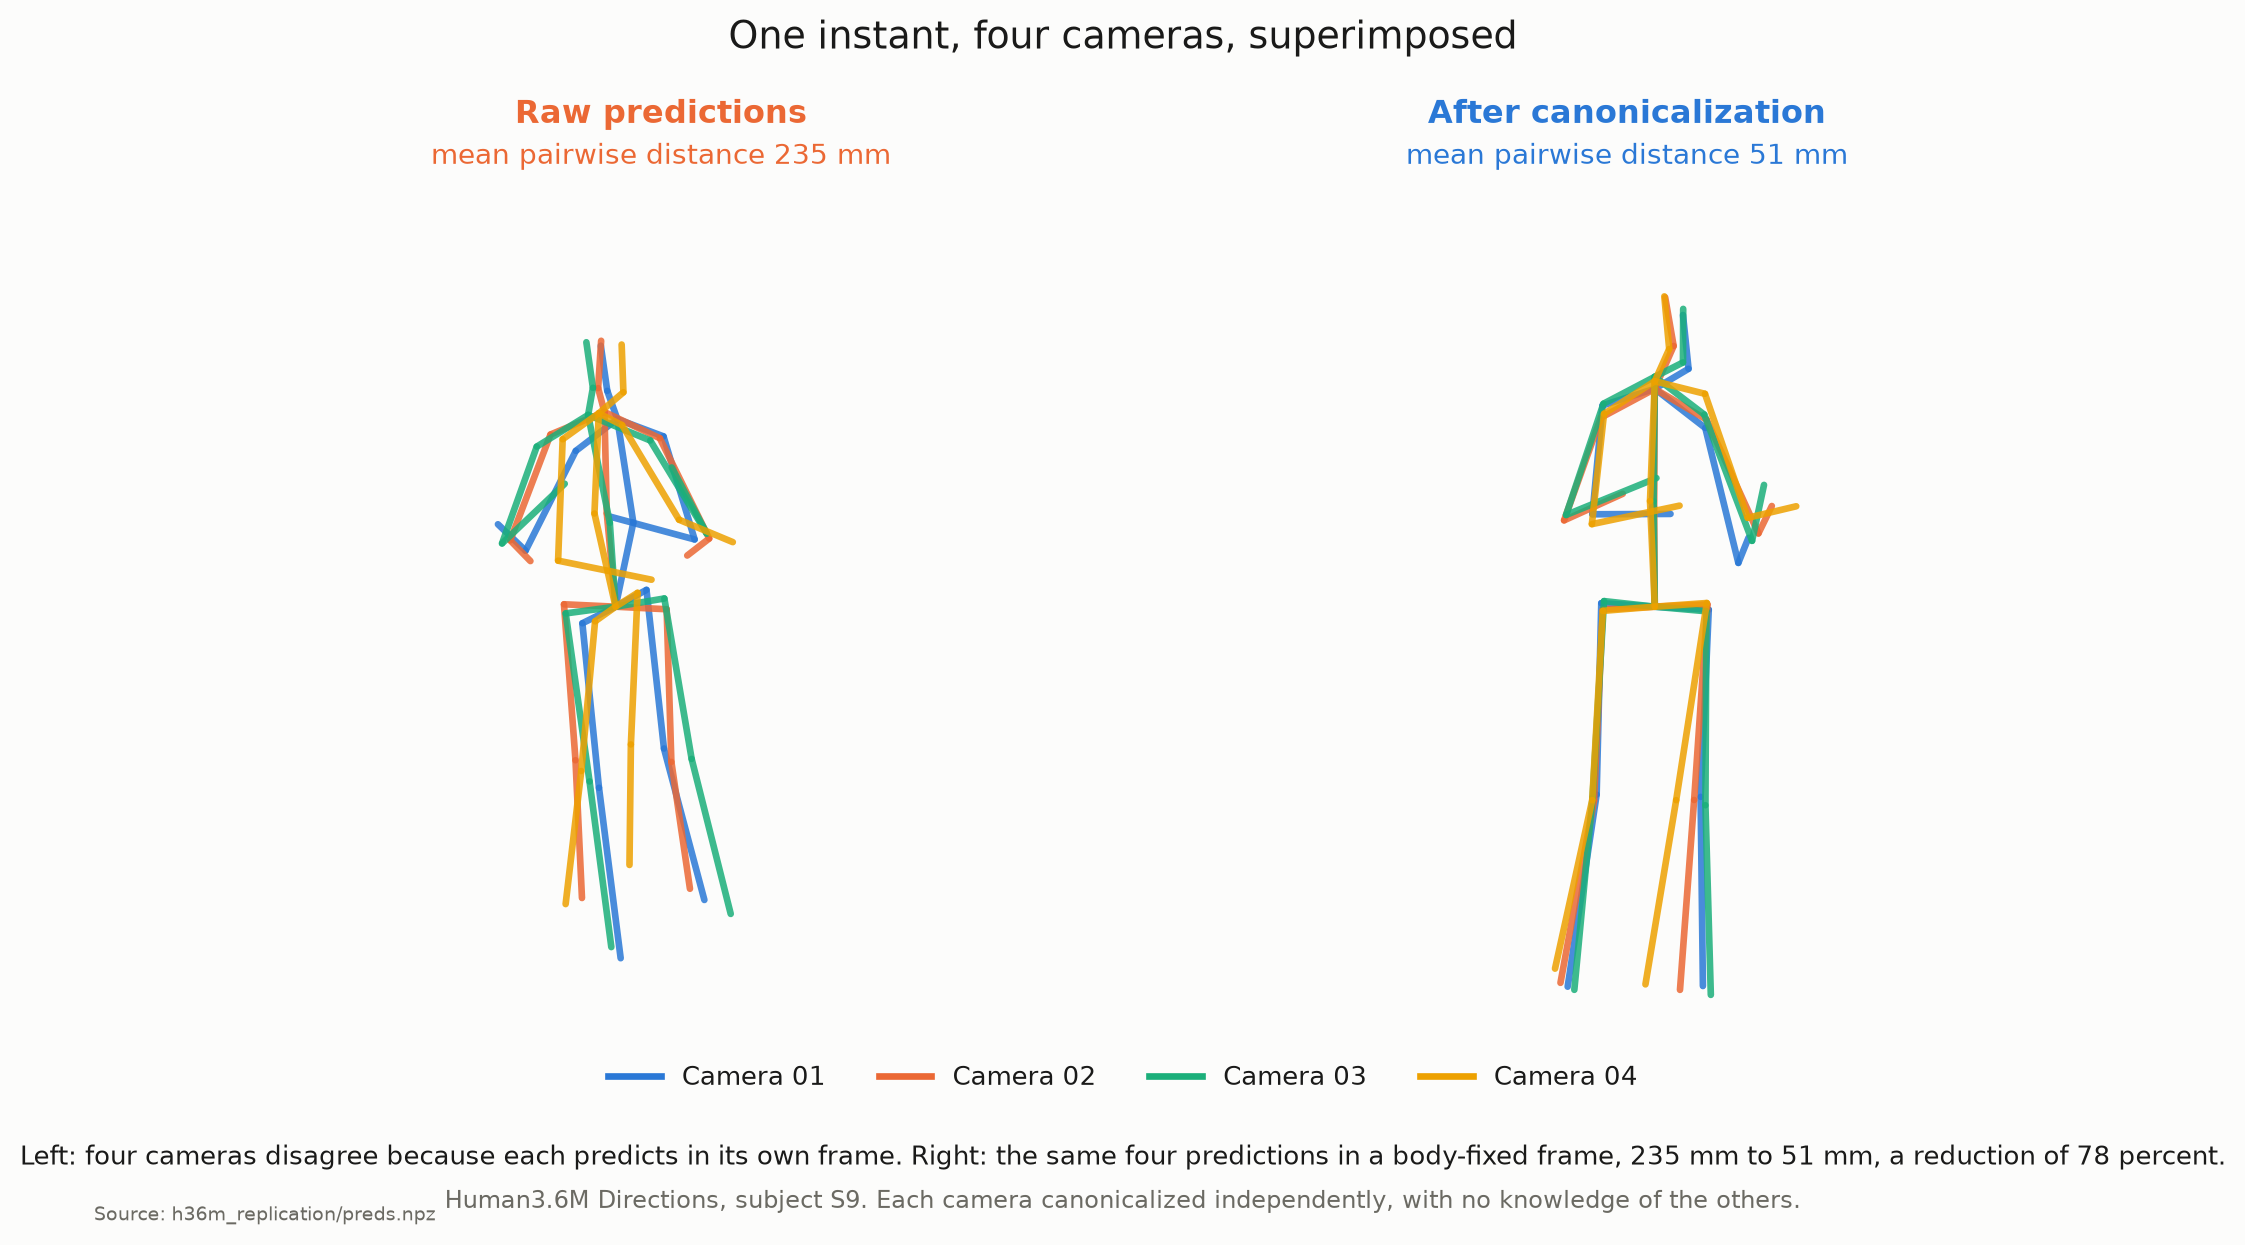
\includegraphics[width=\textwidth]{images/fig_h36m_explainer.png}
\caption{One instant of Human3.6M seen by four synchronized cameras, superimposed. Left: the four raw predictions, which disagree because each is expressed in the frame of its own camera. Right: the same four predictions after canonicalization, each computed independently and without knowledge of the others.}
\label{fig:h36mexplain}
\end{figure}

Figure \ref{fig:h36mexplain} shows what the aggregate hides. Four cameras observing one instant produce four sets of coordinates that visibly disagree, and the same four predictions in a body-fixed frame very nearly coincide, at 235 mm and 51 mm respectively on that frame. No camera has any knowledge of the others at any point.

\begin{figure}[h]
\centering
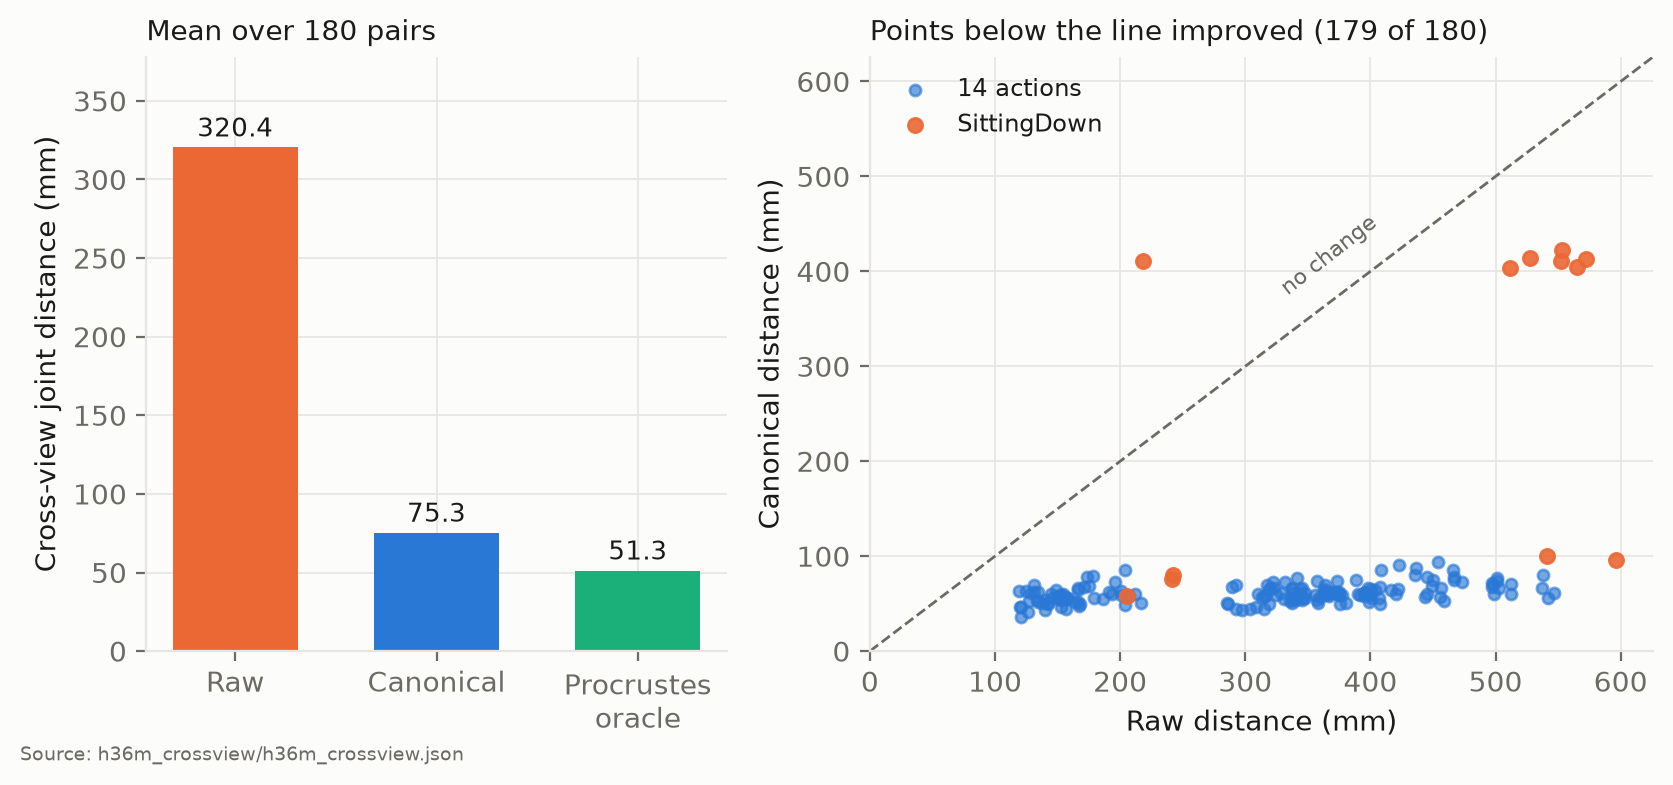
\includegraphics[width=\textwidth]{images/fig_h36m_distances.png}
\caption{Cross-view distance on Human3.6M. Left: means over all 180 held-out pairs. Right: every pair individually, with the diagonal marking no change. Canonical distance collapses to a narrow band irrespective of how far apart the two raw predictions were, except on SittingDown.}
\label{fig:h36mdist}
\end{figure}

The right panel of Figure \ref{fig:h36mdist} shows why the mean is not carried by a few easy pairs. Raw distance varies from roughly 120 mm to 600 mm across pairs, and canonical distance is almost flat across that range at between 40 mm and 100 mm. The reduction therefore does not depend on how far apart the two viewpoints happened to be, which is the behaviour a frame construction should exhibit if it is genuinely removing viewpoint rather than partially compensating for it.

The result holds on both subjects. Subject S11 improves on all ninety of its pairs, from 21.2 percent to 89.7 percent, and subject S9 improves on eighty-nine of ninety. Fourteen of the fifteen actions improve on every one of their twelve pairs, with canonical distances between 45.3 mm and 79.6 mm, as Figure \ref{fig:h36macts} shows.

\begin{figure}[h]
\centering
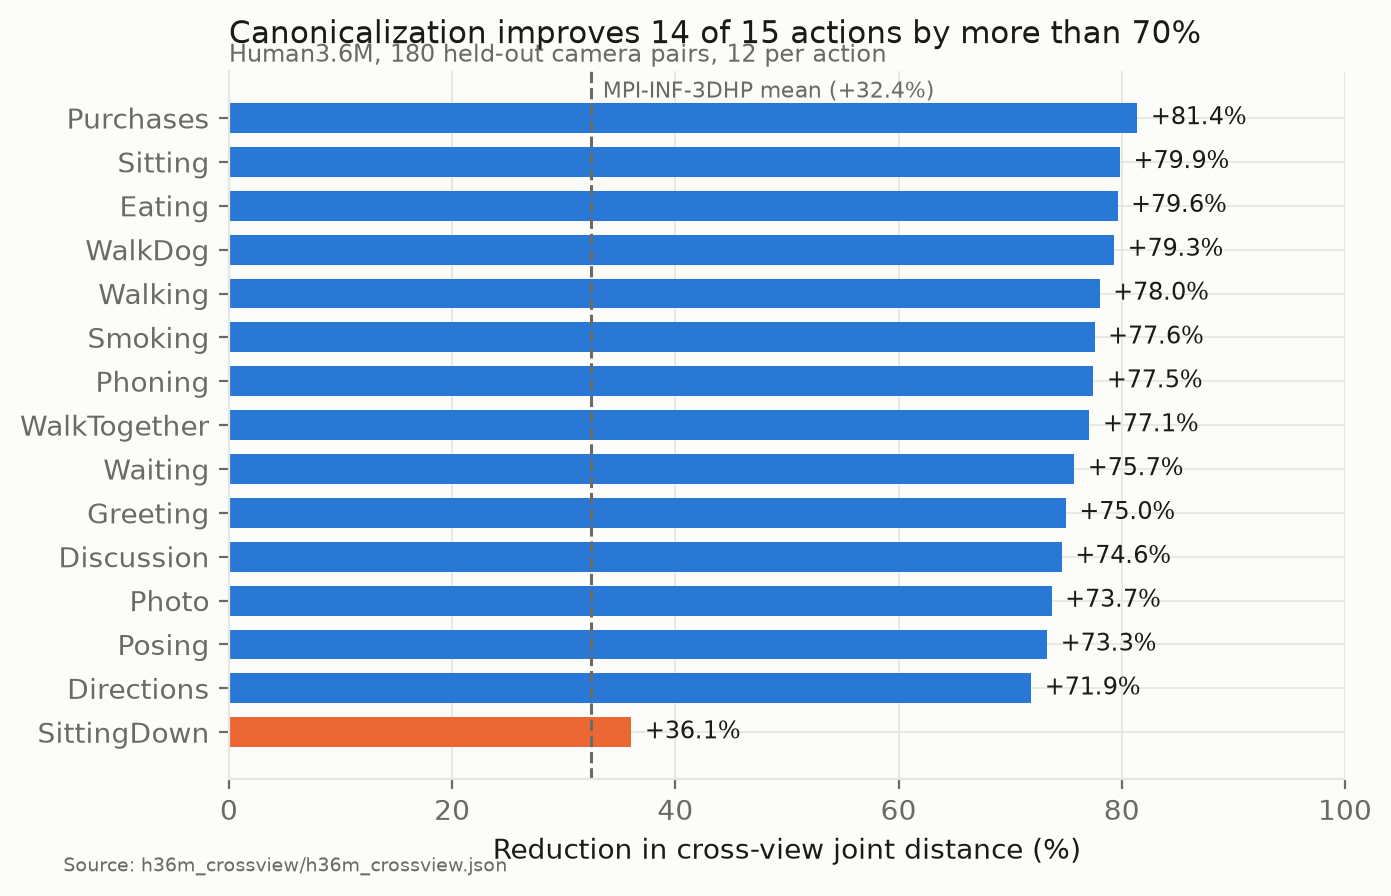
\includegraphics[width=0.92\textwidth]{images/fig_h36m_actions.png}
\caption{Per-action improvement on Human3.6M. Every action except SittingDown exceeds the mean improvement obtained on MPI-INF-3DHP by more than a factor of two.}
\label{fig:h36macts}
\end{figure}

The single exception is informative rather than embarrassing. All twelve SittingDown pairs carry a mean canonical distance of 274.1 mm, far above every other action, and SittingDown contains the one pair in 180 that regresses. SittingDown is also the action on which the backbone itself is least accurate, at 66.4 mm against a mean of 45.1 mm across actions. The body frame is constructed from the predicted torso and hip axes, so a pose the backbone estimates badly yields a frame estimated badly, and the error compounds rather than cancels.

We tested the competing explanation and rejected it. A seated subject might plausibly foreshorten the pelvis and leave the hip axis too short to define a stable frame, which is what we first supposed. Measured across the fifteen actions, the hip axis of SittingDown is 285.3 mm, the second longest of any action, while the shortest belongs to WalkDog at 268.4 mm, which canonicalizes at 79.3 percent without difficulty. The angle between the hip and torso axes is 86.0 degrees for SittingDown, inside the 83 to 88 degree band spanned by every action, so the frame is not ill-conditioned. Neither the length nor the conditioning of the axes distinguishes this action; only the accuracy of the pose they are built from does. Figure \ref{fig:h36msit} puts both candidate explanations on the same axes. Canonical distance is uncorrelated with hip-axis length across the fifteen actions, at $-0.03$, and correlates with the backbone's own accuracy at $+0.76$. That second association survives deleting SittingDown itself, at $+0.70$ over the remaining fourteen actions, so it describes a trend across actions rather than the influence of one outlier.

The failure is therefore inherited from the estimator rather than produced by the frame. This is a sharper statement than the one we began with and a less comfortable one, since a better frame construction cannot repair it.

\begin{figure}[h]
\centering
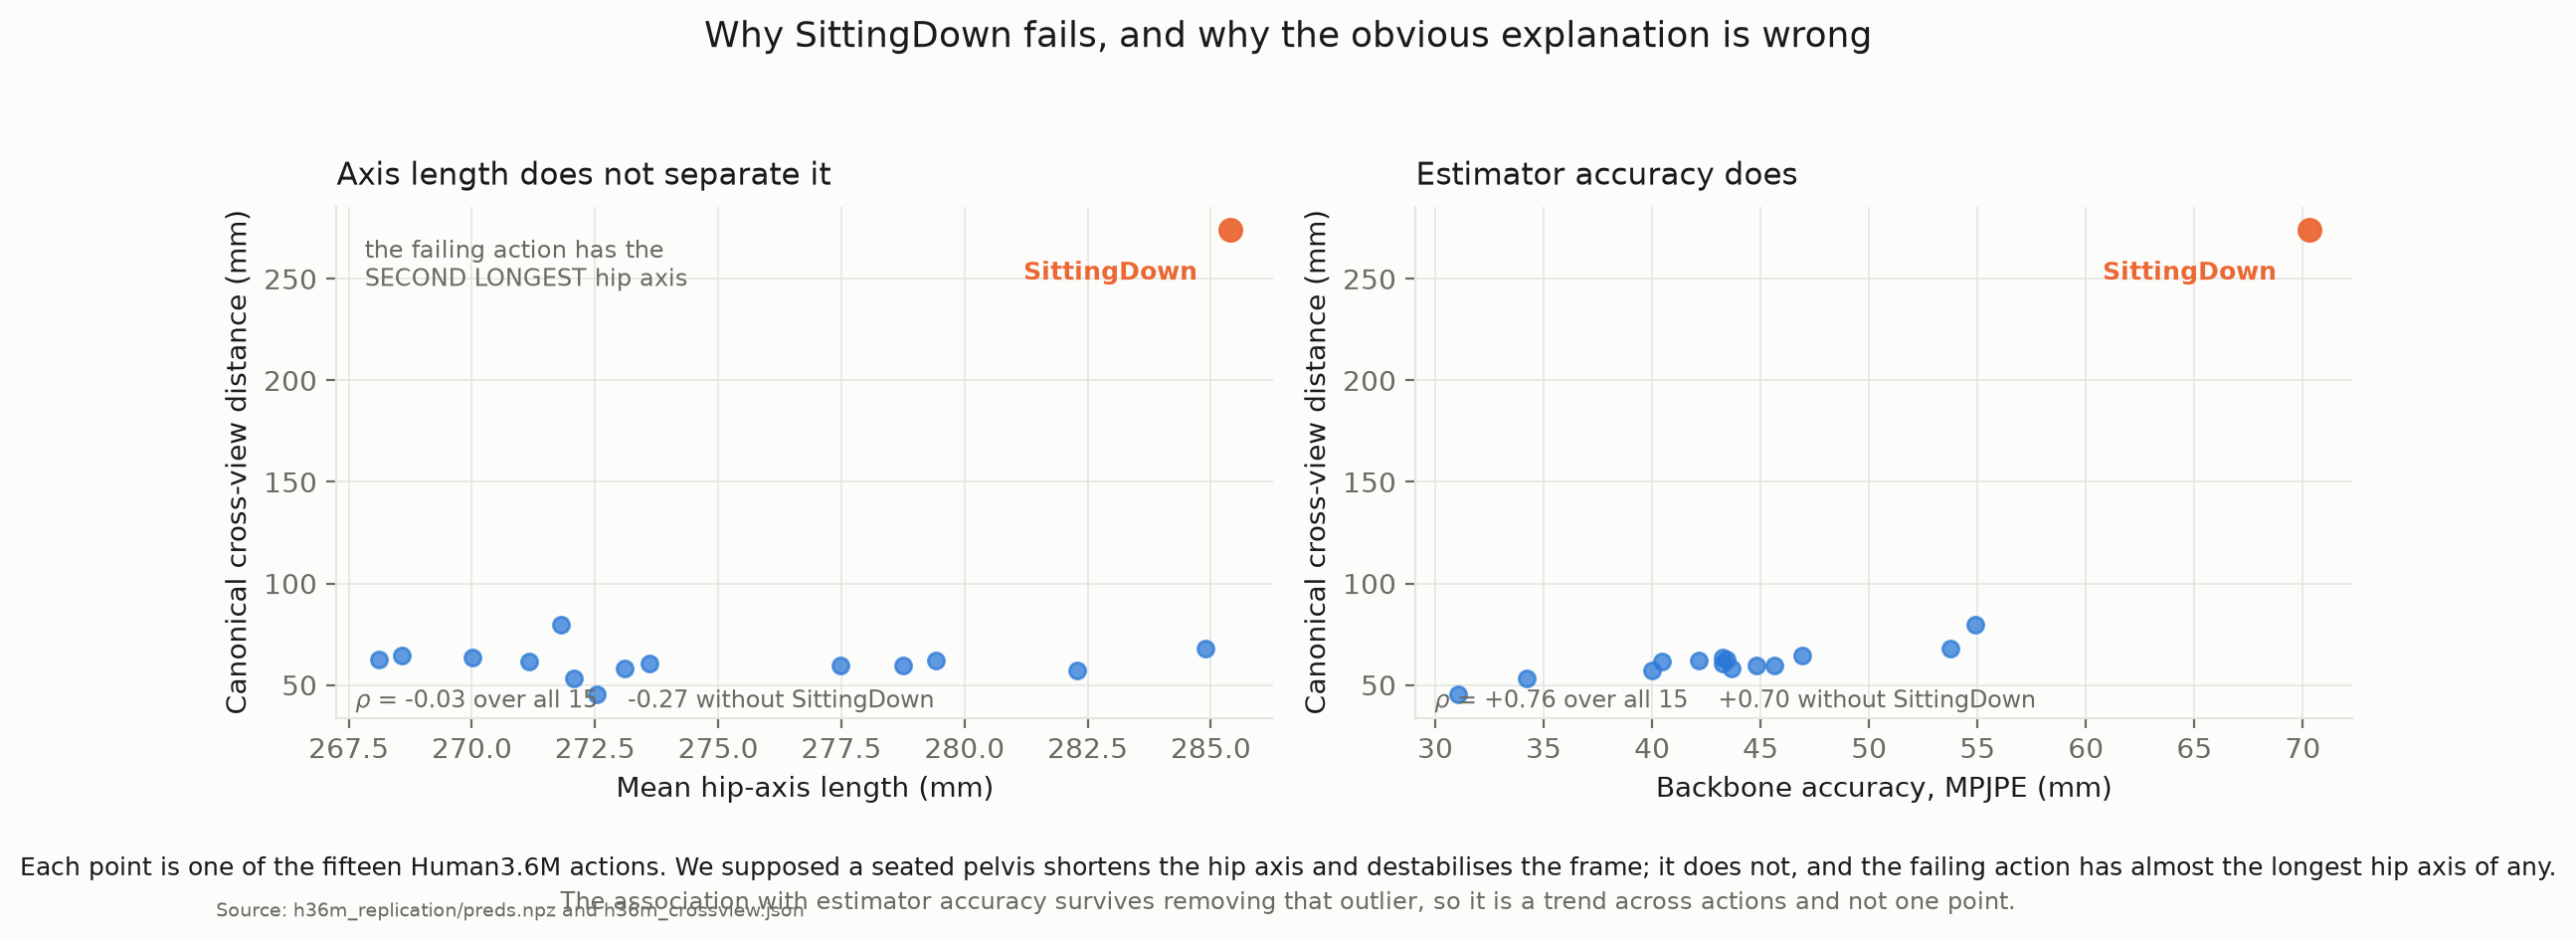
\includegraphics[width=\textwidth]{images/fig_h36m_sittingdown.png}
\caption{Two candidate explanations for the SittingDown result, tested against the fifteen actions. Axis length does not separate the failing action, which has almost the longest hip axis of any. Estimator accuracy does, and the association holds when the failing action is removed.}
\label{fig:h36msit}
\end{figure} The regressing pair additionally had an unusually small raw distance of 218.4 mm against roughly 550 mm for the other pairs of that action, which left little to gain and much to lose. That is the near-aligned camera pair behaviour reported on MPI-INF-3DHP in Section \ref{sec:crossview}, now observed on a second dataset.

We draw one further observation from placing this section beside Section \ref{sec:h36m}. The bone-length signal failed on Human3.6M because the backbone is accurate there, and canonicalization succeeds on Human3.6M for the same reason. Both depend on the quality of the predicted skeleton, and they depend on it in opposite directions.

\section{Calibration-Free Fusion on Human3.6M}
\label{sec:h36mfuse}

We apply the same treatment to multi-view fusion, using the four synchronized cameras as four uncalibrated views. The baseline is the expected error of an arbitrary single view, which is what a deployment with one uncalibrated camera obtains. Every pose is scored by the similarity-aligned distance used throughout this report, which removes rotation and therefore denies any advantage to a pose merely for living in a convenient frame. What canonicalization supplies is the ability to average at all.

Fusion replicates, but only with a robust estimator, and the qualification is the finding. A coordinate-wise median across the four canonical views reduces error from 37.8 mm to 34.6 mm, an improvement of 8.4 percent with a cluster bootstrap interval of $[+2.1, +13.7]$ percent over the thirty videos. The mean across the same four views gives 39.1 mm, a point estimate of $-3.4$ percent whose interval is $[-21.5, +10.5]$ percent. The oracle that selects the best view using ground truth reaches 27.4 mm.

Those intervals discipline the claim in two directions and we state both. The median's advantage is real, since its interval excludes zero. The mean's apparent harm is not established, since its interval does not: the point estimate is negative but the evidence does not distinguish it from no effect, and it would be an overreach to report that an unweighted mean damages accuracy. What the data support is the weaker and more useful statement that the median is reliably beneficial while the mean is not reliably anything.

The instability of the mean is itself informative. Per frame, it improves on the single-view baseline in 67.9 percent of cases, so the typical frame does benefit. Its aggregate is dragged down, and its interval widened, by a minority of catastrophic frames that averaging propagates and a median discards. On MPI-INF-3DHP up to eight views were fused, where one bad view contributes an eighth of the average; with four views it contributes a quarter. We therefore refine rather than retract the fusion claim: canonicalization enables calibration-free fusion, and the estimator must be robust when the number of views is small.

One consequence deserves emphasis, because it bears on the reliability score. The plain median uses no reliability score, no weights and no learned parameters, and at 34.6 mm it outperforms the reliability-weighted mean at 36.6 mm. The weighted mean's own interval, $[-8.4, +12.3]$ percent, includes zero, so weighting by the reliability score does not demonstrably improve on using one arbitrary camera. The sixth independent result concerning that score is that discarding it entirely is better than using it. Figure \ref{fig:h36mfuse} shows the ordering.

\begin{figure}[h]
\centering
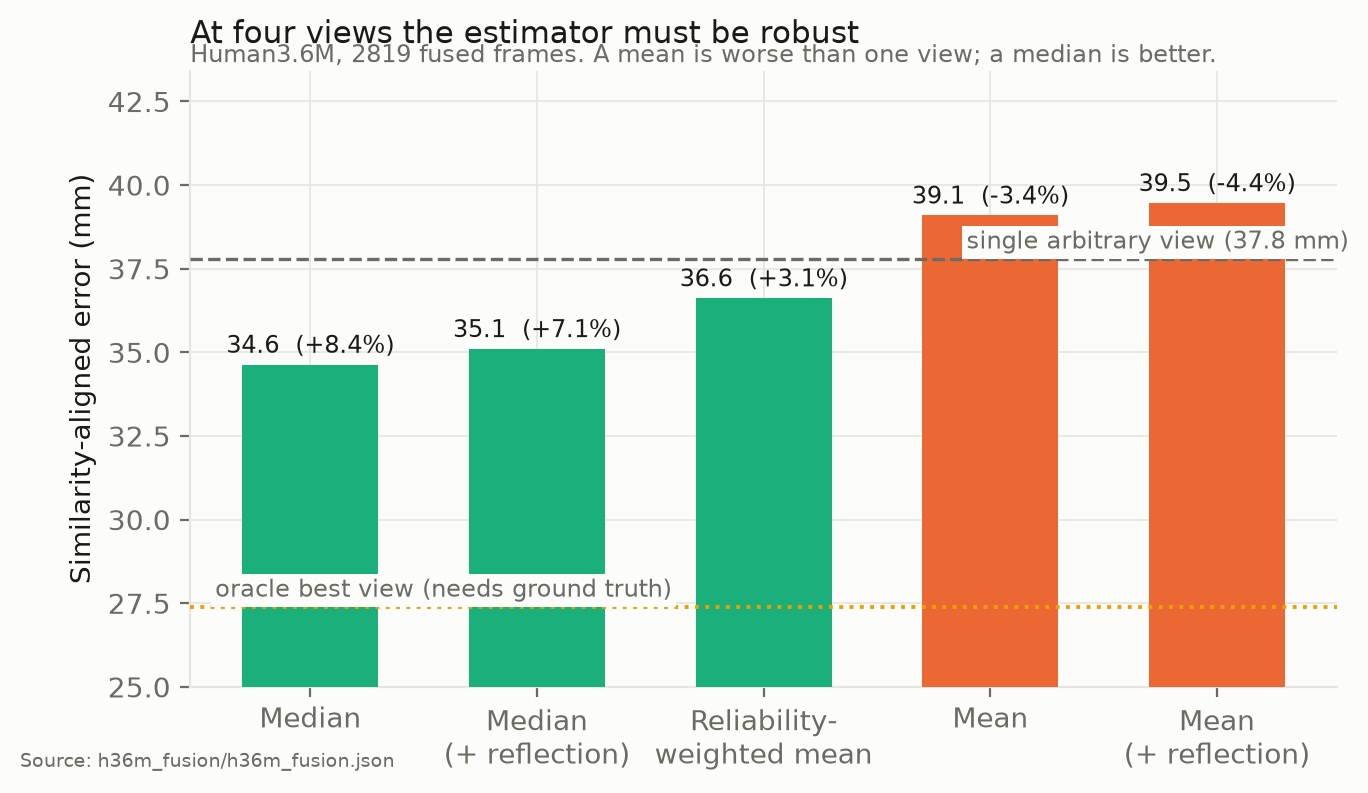
\includegraphics[width=0.95\textwidth]{images/fig_h36m_fusion.png}
\caption{Fusion strategies on Human3.6M. Bars below the dashed line beat an arbitrary single view. Every strategy shown is training-free and label-free, and the best of them uses no reliability score.}
\label{fig:h36mfuse}
\end{figure}

\section{Multi-Scale Per-Limb Canonicalization on Human3.6M}
\label{sec:h36mms}

The multi-scale extension is the third component to receive the cross-dataset treatment. We compare the combined per-limb distance against the global frame on the same 180 held-out pairs, taking both quantities from the same code path so that the baseline and the treatment differ only in the frame used.

The extension replicates. Multi-scale reduces the combined cross-view distance from 62.7 mm to 46.2 mm, an improvement of 25.6 percent with a cluster bootstrap interval of $[+23.6, +27.6]$ percent, and improves 179 of the 180 pairs. No segment fell back to the global frame on any evaluated pose, so the per-limb frames are well conditioned throughout. The improvement is largest exactly where the global frame is weakest: SittingDown gains 32.9 percent on all twelve of its pairs, against 17.8 percent for Walking. This is the expected relationship, since a limb frame is built from that limb's own joints and does not inherit the error in the torso and hip axes that Section \ref{sec:h36mcv} identified as the cause of the SittingDown result.

\subsection{A Bilateral Asymmetry, and What Caused It}

The per-level breakdown revealed a defect in our own implementation that the MPI-INF-3DHP evaluation had not exposed. The two arms agree closely, at 57.1 mm and 57.6 mm, which is what bilateral symmetry predicts for a subject performing symmetric everyday actions. The two legs do not: the right leg scores 69.4 mm against 30.7 mm for the left, a factor of 2.3. We note that the segment keys in our implementation are mirrored with respect to anatomy, so the key named \texttt{left\_leg} holds the joints of the anatomical right leg. Anatomical names are used throughout this section and in Table \ref{tab:msfix}; the mirroring affects labels only and no geometry or number depends on it.

Inspecting the segment definitions explains it. Both arms take the thorax-to-shoulder vector as primary axis and the shoulder-to-elbow vector as secondary. The legs were defined inconsistently with each other: the left leg takes hip-to-knee as primary and knee-to-ankle as secondary, while the right leg takes root-to-hip as primary and hip-to-knee as secondary. The root-to-hip vector is roughly half a hip width, whereas hip-to-knee is a full thigh. Section 3.2 argues that frame sensitivity to joint error scales inversely with the length of the defining vector, so the right leg was predicted to be the noisier of the two before the cause was found, and for exactly this reason.

We tested the correction rather than assuming it. Defining both legs identically, with hip-to-knee as primary and knee-to-ankle as secondary, gives the middle column of Table \ref{tab:msfix}. The right leg falls from 69.4 mm to 29.3 mm, which brings it into agreement with the left leg at 30.7 mm. Every other level is unchanged to the reported precision, which is the signature of a correct diagnosis rather than a general perturbation. The combined distance falls from 46.2 mm to 39.1 mm, the improvement over the global frame rises from 25.6 percent to 37.2 percent, and all 180 pairs now improve rather than 179.

\subsection{The Same Defect in Both Arms}

Applying the diagnosis consistently exposes a second instance of it. Both arms take the thorax-to-shoulder vector as primary axis, which is about half a shoulder width, where the corrected legs take a full thigh. The bilateral comparison could not reveal this, because both arms share the defect and therefore agree with each other at 57.1 mm and 57.6 mm. Agreement between two measurements is not evidence that either is correct, and here it actively concealed the problem: the arms looked healthy precisely because they were equally affected.

Rebuilding both arms from their own long segments, shoulder-to-elbow as primary and elbow-to-wrist as secondary, produces the largest single improvement in this chapter. The right arm falls from 57.1 mm to 26.8 mm and the left from 57.6 mm to 26.3 mm. The combined multi-scale distance falls to 28.2 mm, the improvement over the global frame reaches 55.1 percent with a cluster bootstrap interval of $[+53.6, +56.5]$ percent, and all 180 pairs improve with no segment falling back to the global frame.

The corrected levels support the diagnosis independently of the improvement they produce. All five now lie between 26.3 mm and 30.7 mm, where before they ranged from 28.6 mm to 69.4 mm. A construction applied consistently to five anatomically different segments should give five similar numbers, and it now does. That convergence was not optimized for, since each segment was redefined by the same rule rather than tuned, and it is the strongest evidence that axis length, not anatomy, was driving the spread.

\begin{table}[h]
\centering
\caption{Building every segment frame from that segment's own long axis. Bold entries changed from the column to their left.}
\label{tab:msfix}
\begin{tabular}{lrrr}
\hline
\textbf{Level} & \textbf{As implemented} & \textbf{Legs alike} & \textbf{Arms also} \\
\hline
Global frame & 62.7 mm & 62.7 mm & 62.7 mm \\
Torso & 28.6 mm & 28.6 mm & 28.6 mm \\
Right arm & 57.1 mm & 57.1 mm & \textbf{26.8 mm} \\
Left arm & 57.6 mm & 57.6 mm & \textbf{26.3 mm} \\
Right leg & 69.4 mm & \textbf{29.3 mm} & 29.3 mm \\
Left leg & 30.7 mm & 30.7 mm & 30.7 mm \\
\hline
Combined multi-scale & 46.2 mm & \textbf{39.1 mm} & \textbf{28.2 mm} \\
Improvement over global & +25.6\% & \textbf{+37.2\%} & \textbf{+55.1\%} \\
95\% CI & $[+23.6, +27.6]$ & --- & $\mathbf{[+53.6, +56.5]}$ \\
Pairs improved & 179 / 180 & \textbf{180 / 180} & \textbf{180 / 180} \\
\hline
\end{tabular}
\end{table}

\begin{figure}[h]
\centering
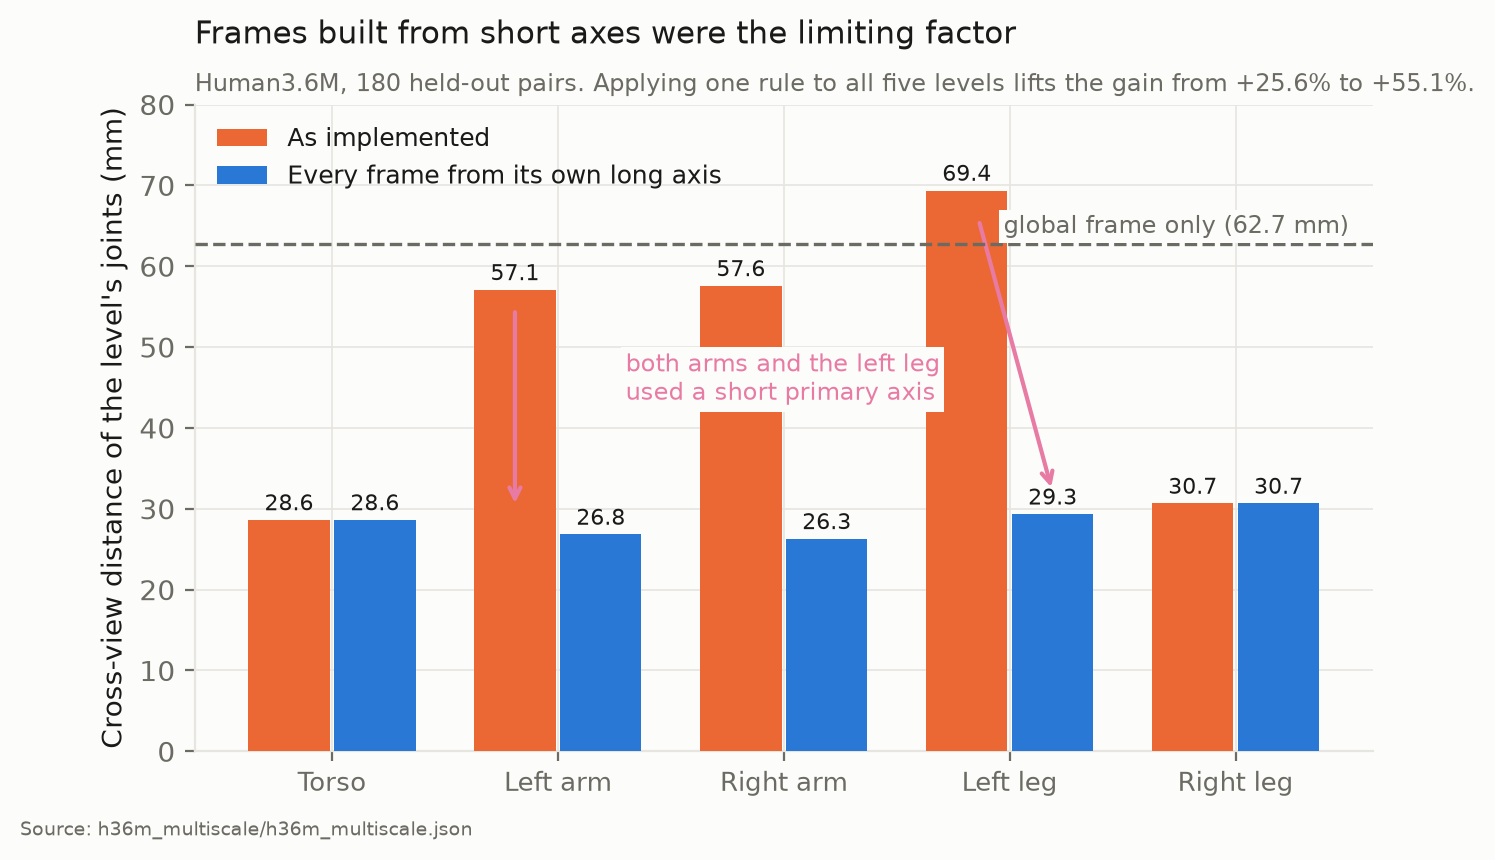
\includegraphics[width=0.97\textwidth]{images/fig_h36m_multiscale.png}
\caption{Per-level cross-view distance on Human3.6M. Three of the five frames were built from an axis roughly half a shoulder or hip width long; rebuilding them from the segment's own long axis halves their cross-view distance and brings all five levels into a 4.4 mm band.}
\label{fig:h36mms}
\end{figure}

Two remarks are in order. The first concerns what the correction is not: it adds no parameters, consumes no labels and changes no algorithm, since it only makes two segment definitions agree with each other and with the four that were already consistent. The second concerns why it went unnoticed. The MPI-INF-3DHP evaluation reported one combined number per camera pair and confirmed that multi-scale beat the global frame, which it did. The defect was invisible at that granularity and became obvious only when the levels were reported separately on a dataset large enough for the bilateral comparison to be unambiguous. We report the corrected figures as a variant rather than as the headline, because the MPI-INF-3DHP results elsewhere in this chapter were produced with the original definitions and we have not re-run them.

\section{A Second Backbone}
\label{sec:backbone2}

The framework consumes a seventeen by three array and nothing else, so independence from the estimator is structural. It was not, until this section, empirical. We test it by replacing the backbone and changing nothing else.

MotionBERT is a suitable second choice because it shares almost nothing with the first. It is a dual-stream spatio-temporal transformer of 42.5 million parameters against a 2.24 million parameter transformer and graph-convolution hybrid, a factor of nineteen in size and a different architecture family. We run it over the same clips, with the same windows, and pass its predictions to the same three evaluation modules. Not one line of those modules changes; they take an argument naming a different cache, and that argument is the entire adaptation. A trained canonicalizer would at minimum require validation against the new output distribution, and in general retraining.

One caveat belongs here. The released MotionBERT checkpoint is fine-tuned at 243 frames and we evaluate it at 27, so it runs below its published accuracy. It reaches 44.03 mm on these clips where its paper reports 37.5 mm at the longer window. We hold the window identical rather than favourable because the backbone must be the only variable, and at 44.03 mm against 45.15 mm the two backbones are close enough in accuracy that no result below can be attributed to one being weaker.

All three components replicate, as Table \ref{tab:backbone} shows. Canonicalization improves every one of the 180 pairs rather than 179, at 77.5 percent with an interval of $[+76.6, +78.5]$, and closes 94.5 percent of the oracle gap. Multi-scale gives 24.5 percent against 25.6 percent, and under the corrected long-axis definitions 54.9 percent against 55.1 percent, a difference of two tenths of a percentage point across a nineteen-fold change in model size. Fusion behaves as before: the median improves on an arbitrary view at 6.8 percent with an interval excluding zero, while the unweighted mean and the reliability-weighted mean do not.

\begin{table}[h]
\centering
\caption{The same framework over two unrelated backbones, with no code changed.}
\label{tab:backbone}
{\fontsize{10}{12}\selectfont
\begin{tabular}{lrr}
\hline
 & \textbf{MotionAGFormer-XS} & \textbf{MotionBERT} \\
 & 2.24M, hybrid & 42.5M, transformer \\
\hline
Accuracy on these clips & 45.15 mm & 44.03 mm \\
\hline
Cross-view improvement & +74.1\% & \textbf{+77.5\%} \\
95\% CI & $[+69.8, +77.2]$ & $[+76.6, +78.5]$ \\
Pairs improved & 179 / 180 & \textbf{180 / 180} \\
Oracle gap closed & 90.5\% & 94.5\% \\
Frame validity & 100\% & 100\% \\
\hline
Multi-scale, as implemented & +25.6\% & +24.5\% \\
Multi-scale, own long axis & +55.1\% & +54.9\% \\
\hline
Fusion, median & +8.4\% & +6.8\% \\
Fusion, unweighted mean & $-3.4\%$, spans zero & $-10.2\%$, spans zero \\
Reliability-weighted mean & $+3.1\%$, spans zero & $-1.8\%$, spans zero \\
\hline
\end{tabular}}
\end{table}

The per-action breakdown settles a question Section \ref{sec:h36mcv} could only argue. SittingDown, the single action on which canonicalization failed, carries a canonical distance of 274.1 mm under the first backbone and 87.5 mm under the second. Every other action moves by at most five millimetres between the two. If the failure were a property of the body frame it would survive a change of estimator, because the frame construction is byte-identical in both runs. It does not survive. That is direct evidence for the conclusion Section \ref{sec:h36mcv} reached from correlations alone: the failure is inherited from the estimator, and a better estimator removes it.

We therefore state model independence as a measurement rather than an argument. The same code, unmodified, improves 359 of 360 camera pairs across two backbones that share no architecture.

\section{Testing the Axis-Length Principle on the Global Frame}
\label{sec:multilandmark}

Section \ref{sec:h36mms} established that a frame's cross-view consistency is governed by the length of the axis it is built from, and Section \ref{sec:backbone2} showed that result reproduces to two tenths of a percentage point on an unrelated backbone. Both were obtained on per-limb frames. The global frame was never revisited, and it uses the shorter of the two lateral vectors available: the hip axis measures 271.6 mm against 295.2 mm for the shoulder axis, over 2672 poses. The principle therefore makes a prediction about our own method that we had not tested.

We pre-registered that prediction before running anything, in the manner of Section \ref{sec:relfails}, and committed it separately so that version history shows the criterion preceding the number. The pass condition was that a multi-landmark estimate beat the two-vector baseline with a cluster bootstrap interval excluding zero on \emph{both} backbones. Five variants were compared on identical frames, with a shared validity mask so the comparison is paired.

Two lateral estimates can be combined only because they point the same way. The hip vector runs from the right hip to the left and the shoulder vector from the right shoulder to the left, and their cosine is $+0.969$ with the same sign on every one of the 2672 poses measured. Weighting is derived rather than tuned: if per-joint noise is fixed and angular error scales as the inverse of segment length, variance scales as the inverse square, so inverse-variance weighting gives a weight equal to the squared length and introduces no free parameter.

\begin{table}[h]
\centering
\caption{Global frame from redundant landmarks. Paired gain is against the two-vector baseline on identical frames.}
\label{tab:multilandmark}
{\fontsize{10}{12}\selectfont
\begin{tabular}{lrrrr}
\hline
 & \multicolumn{2}{c}{\textbf{MotionAGFormer-XS}} & \multicolumn{2}{c}{\textbf{MotionBERT}} \\
\textbf{Lateral axis from} & \textbf{mm} & \textbf{gain 95\% CI} & \textbf{mm} & \textbf{gain 95\% CI} \\
\hline
Hips (the current frame) & 75.3 & --- & 60.1 & --- \\
Hips alone & 74.9 & $[-4.8, +5.6]$ & 59.7 & $[+0.3, +0.5]$ \\
\textbf{Shoulders alone} & \textbf{71.4} & $\mathbf{[+1.6, +7.8]}$ & \textbf{57.5} & $\mathbf{[+1.7, +3.6]}$ \\
Both, length-weighted & 72.0 & $[-1.8, +8.3]$ & 61.5 & $[-12.0, +4.3]$ \\
Spine chain by SVD & 72.7 & $[+0.4, +6.1]$ & 68.9 & $[-25.1, +2.2]$ \\
\hline
\end{tabular}}
\end{table}

The pre-registered criterion fails, and the shape of the failure is more useful than a pass would have been. Table \ref{tab:multilandmark} separates two things that we had treated as one. Replacing the hip axis with the longer shoulder axis improves the global frame on both backbones, by 5.2 and 4.4 percent, with intervals excluding zero in each case. That is the axis-length principle operating exactly as stated, now confirmed at the global scale on two estimators. Combining the two lateral axes, however, does not help. The weighted estimate is indistinguishable from the baseline on the first backbone and worse on the second, and the spine-chain estimate is worse still, losing 8.8 mm on MotionBERT.

We take the natural reading, which the pre-registration named in advance as the expected failure mode. Redundancy pays only when the redundant estimates carry independent errors. Here they do not: the hip and shoulder positions are produced by one network from one image, so their errors are correlated through the shared prediction, and averaging them reduces nothing while diluting the longer and better-conditioned of the two. The spine-chain variant fails hardest because it is the most redundant, drawing a single direction from five joints that the estimator places with correlated error.

\subsection{Testing the Predicted Law}

Section \ref{sec:axistheory} derives $d^{2} \approx (c\,\bar{r}/L)^{2} + d_0^{2}$ from noise propagation, which is a stronger statement than the ordering we have been asserting, and testable. We fit it by least squares to the eight limb-frame definitions of Section \ref{sec:h36mms}, which apply one construction to anatomically different segments and so span a genuine range of $\bar{r}/L$, and we repeat the fit independently on both backbones. Two parameters are fitted to eight points.

The verdict is mixed and we state both halves. The monotone prediction holds strongly and reproduces: the rank correlation between $\bar{r}/L$ and measured cross-view distance is $+0.904$ on the first backbone and $+0.880$ on the second. More tellingly, the fitted constants agree across two independently trained networks of different architecture and nineteen-fold different size, at $c = 21.3$ and $21.5$ mm, implying a per-joint noise of $\sigma = 7.5$ and $7.6$ mm. Two unrelated estimators returning the same physical constant to within one percent is not something an accidental correlation produces, and it is the strongest evidence we have that the mechanism in equation \eqref{eq:theta} is the operative one.

The functional form, however, is too simple. The fit explains 70 percent of the variance and predicts held-out definitions poorly, with a leave-one-out mean absolute error of 16 mm against observations spanning 26 to 69 mm, and it systematically over-predicts the best-conditioned frames. At least three of its assumptions are visibly wrong: per-joint noise is not uniform, since wrists and ankles are far less reliable than hips and shoulders; the two views' errors are not fully independent, since both come from one detector with shared biases; and the small-angle approximation weakens exactly where the frame is worst.

We therefore claim the mechanism and not the equation. Axis length governs frame stability, the direction and the constant are reproducible across backbones, and the specific inverse law is a first-order account that should not be quoted as a predictive model.

The practical consequence is small and concrete. The best available global frame among those tested is not a multi-landmark estimate but the existing construction with one vector exchanged for a longer one, a change of two joint indices. We report it as a measured improvement rather than adopting it in the results above, which were computed with the original definition throughout, and we note that the corresponding change to the segment frames in Section \ref{sec:h36mms} was validated on Human3.6M only. Re-running both datasets under the corrected definitions is the cheapest outstanding item in this report.

\section{Ablation with Abstention}

Table \ref{tab:ablation} reports the three conditions on the development pair and Figure \ref{fig:coverage} traces error against coverage as the abstention threshold varies. Coverage is reported alongside error throughout, since an abstaining method could otherwise report an arbitrarily low error by answering arbitrarily rarely.

\begin{table}[h]
\centering
\caption{Three conditions on the development pair}
\label{tab:ablation}
\begin{tabular}{|l|c|c|}
\hline
\textbf{Condition} & \textbf{Distance} & \textbf{Coverage} \\
\hline
Raw root-relative & 0.1439 & 100\% \\
\hline
Canonical & 0.1143 & 100\% \\
\hline
Reliability-aware, threshold 0.5 & 0.1044 & 89\% \\
\hline
Reliability-aware, threshold 0.8 & \textbf{0.0904} & 69\% \\
\hline
\end{tabular}
\end{table}

\begin{figure}[h]
\centering
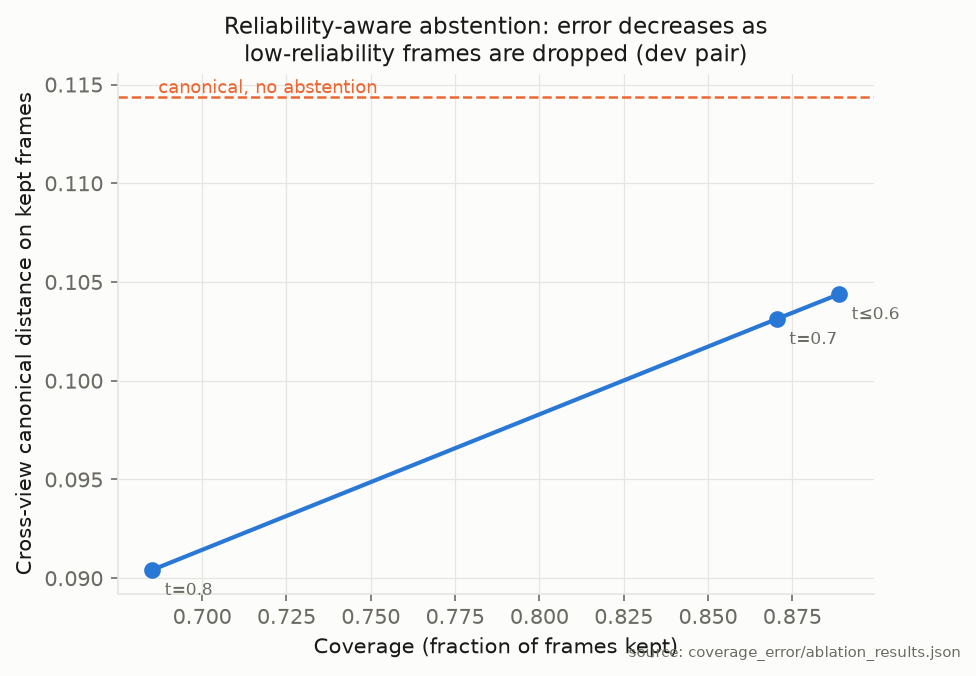
\includegraphics[width=0.68\textwidth]{images/fig_coverage_error.png}
\caption{Coverage against error as the abstention threshold varies}
\label{fig:coverage}
\end{figure}

\section{Negative Result on Cross-View Retrieval}

Canonicalization degrades cross-view retrieval, with recall at rank one falling from 0.02 to 0.00 and mean reciprocal rank falling by 6.9 percent. This outcome is expected, because retrieval across similar standing poses relies in part on viewpoint information, which canonicalization removes by construction. The result delimits the scope of the method rather than undermining it.

% ========================== CHAPTER 5 ================================
\chapter{CONCLUSION AND FUTURE WORK}

In this project we developed a framework that makes the predictions of a frozen monocular 3D pose estimator comparable across viewpoints without training, labels, or camera calibration. Canonicalization reduces cross-view joint distance by 32.4 percent across twenty-seven held-out camera pairs of MPI-INF-3DHP and by 74.1 percent, with a cluster bootstrap interval of $[+69.8, +77.2]$ percent, across 180 held-out pairs of Human3.6M, where it improves 179 of 180 pairs and closes 90.5 percent of the gap to a per-frame Procrustes oracle. The multi-scale extension improves every pair tested on the first dataset and 179 of 180 on the second, and reporting its levels separately showed that the length of the axis a frame is built from governs how consistent that frame is across views. Rebuilding each segment frame from its own long axis raises the gain from 25.6 to 55.1 percent and improves all 180 pairs. The shared frame enables calibration-free multi-view fusion, which on Human3.6M requires a median rather than a mean, because at four views only the median improves reliably on an arbitrary single camera.

It is worth stating plainly what kind of contribution this is. The work is a deployment-oriented geometric framework, not a new learning algorithm. Body-frame normalization is not itself novel, and Section 2.3 says so: 3DPCNet addresses the same problem and reports a hand-built baseline of this kind performing worse than its learned alternative. What we claim is the combination and its evidence. The framework adds zero trained parameters, consumes no labels and requires no calibration, so applying it to a new estimator, camera or domain costs nothing but the arithmetic; and it is evaluated over 209 camera pairs across two datasets, the second of which took no part in its design. Whether that trade is worth making depends on whether a practitioner can afford to train, which is a deployment question rather than an accuracy one.

One finding is genuinely a design result rather than an evaluation. The consistency of a body frame across viewpoints is governed by the length of the axis it is built from, which we predicted from the construction, discovered through a bilateral asymmetry we had not gone looking for, confirmed by correcting it, and then generalized to a second case that the same reasoning identified. It raises the multi-scale improvement from 25.6 to 55.1 percent and costs no parameters. We regard it as the most transferable thing in this report, since any method that builds a frame from anatomical landmarks faces the same choice.

We regard the negative results as equally important. We falsified the analytic reliability score, one of the framework's original components, as a predictor of accuracy along five independent axes, and we identified the cause: within-frame geometric plausibility is invariant to the depth error that dominates monocular estimation. That diagnosis motivated a signal based on a physical invariant which the model cannot satisfy merely by being confidently wrong, and temporal bone-length inconsistency predicts error from a single camera at a Spearman coefficient of $+0.492$ on that dataset. We then replicated the experiment on Human3.6M, where the coefficient falls to $+0.098$ and every criterion fails, and we retract the general claim. What survives is narrower and, we would argue, more useful for being bounded: the signal detects domain shift severe enough to deform the predicted skeleton, and it does not rank the residual depth error of a backbone that is already accurate. The mechanism is the one that defeated the reliability score, extended along the time axis, since bone-length consistency is invariant to a temporally coherent depth error just as within-frame plausibility is invariant to a coherent one.

The methodological contribution may prove as durable as the empirical one. We recompute every claim in this report from stored artifacts using an automated audit, we committed the pass criterion for the test-time augmentation experiment to version control before running that experiment, and we report each retracted claim alongside the evidence that retracted it. The bone-length result is the clearest case. It was our strongest single-view finding, we tested it on a second dataset rather than leaving it as future work, and it did not survive. We report the retraction in the same detail we would have reported a confirmation.

\section*{Limitations}

The framework is intended for deployment-oriented canonicalization of a frozen estimator, not as a replacement for a learned canonicalization network. A method that trains on the deployment distribution has information this one does not and should be expected to use it; the comparison that matters is therefore not accuracy alone but accuracy against what the user must supply. We make no claim to the contrary and none of our experiments test one.

Both datasets are laboratory capture with controlled lighting, a single subject in frame and a fixed camera rig, so neither exercises the uncontrolled conditions where viewpoint quality varies per frame. Four subjects in total appear across the two test splits. Two lifting backbones were evaluated end to end and both were transformer-based; a convolutional or diffusion estimator might behave differently, and the second backbone ran below its published accuracy because we held the temporal window fixed. Near-aligned camera pairs gain little and may regress, which we observe on both datasets. Fusion by an unweighted mean is unsafe at four views, and we did not determine the number of views at which it becomes safe. Canonicalization degrades where the backbone itself degrades, as SittingDown shows, so the method inherits rather than repairs the failure modes of the estimator it wraps. The abstention threshold was fixed at implementation time rather than calibrated, and the framework offers no coverage guarantee of the kind conformal methods provide. The bone-length signal was discovered by exploratory analysis rather than pre-registered, which is the practice its failure to replicate argues against.

\section*{Future Work}

The results above determine what is worth doing next more sharply than a general wish list would, so we order the following by what each would settle rather than by ambition, and we state what each requires.

\subsection*{Directly Answerable With Present Resources}

\noindent \textbf{A second frozen backbone.} The framework consumes any 17 by 3 pose, so model independence is structural, but Section 6 lists its absence as a limitation because we have not demonstrated it. Running the identical modules over MotionBERT, a 42.5 million parameter transformer architecturally unlike the 2.2 million parameter hybrid used here, would convert the argument into a measurement. The requirement is one inference pass; no part of the framework would change, and the fact that no part changes is precisely the claim. This is the single most valuable outstanding experiment, because estimator-agnosticism is the axis on which the method is positioned against trained alternatives, and it is currently the least evidenced.

\noindent \textbf{A trained canonicalization head as a control.} We argue that a zero-parameter frame is preferable to a trained one on deployment grounds, and we do not measure what training buys. Training a small rotation-predicting head on the Human3.6M training split and evaluating it on the same 180 held-out pairs would quantify the trade directly. The outcome is informative in both directions: if the trained head wins by a wide margin the deployment argument must carry more weight than it currently does, and if it wins narrowly or not at all the case for the analytic frame strengthens considerably.

\noindent \textbf{The view count at which mean fusion becomes safe.} Section \ref{sec:h36mfuse} shows that an unweighted mean over four views is worse than one arbitrary view while a median is better, and attributes the difference to breakdown point. Subsampling the eight cameras of MPI-INF-3DHP to every count between three and eight would locate the crossover empirically. This is a small experiment with a practical payoff, since a deployment must choose an estimator before it knows how many cameras it will have.

\noindent \textbf{Predicting when the body frame is unreliable.} Section \ref{sec:h36mms} shows that axis length governs the consistency of a frame across segment definitions, and Section \ref{sec:h36mcv} shows that axis length does \emph{not} explain which action fails, since the worst action has the second longest hip axis. Both are measurements of the same quantity pointing in different directions, and the reconciliation is that axis length matters when comparing constructions on the same data, while pose accuracy matters when comparing data under the same construction. A useful abstention rule would need the second, and the second is not computable from geometry alone. Establishing what does predict per-action failure, without labels, is the open problem this leaves.

\noindent \textbf{A frame built from all joints rather than two vectors.} The global frame is determined by the torso and hip axes alone, so an error in either propagates undamped. Estimating the frame from all seventeen joints under a robust criterion, or regularizing it with a subject skeleton accumulated online, should degrade more gracefully. The multi-scale results make this concrete rather than speculative: frames built from longer, better-estimated axes are markedly more consistent across views, and the global frame currently uses one of the shortest axes available.

\noindent \textbf{Re-running MPI-INF-3DHP with the corrected segment definitions.} The segment corrections of Section \ref{sec:h36mms} were validated on Human3.6M only, and the MPI-INF-3DHP multi-scale figures elsewhere in this report were produced with the original definitions. Repeating that evaluation would establish whether the same gain appears on the first dataset. This is the cheapest outstanding item and it would remove an inconsistency in the present report rather than add a new claim.

\subsection*{Requiring Additional Data}

\noindent \textbf{More viewpoints and more subjects.} Both datasets used here are laboratory capture, and four subjects appear across the two test splits. Multi-camera collections with more cameras, such as CMU Panoptic, would test whether the improvement continues to hold as viewpoints become more extreme, and would supply the larger view counts the fusion question above requires. Genuinely uncontrolled footage is a harder proposition than it first appears, because the central claim is about agreement between simultaneous views and most in-the-wild datasets are monocular. Establishing the method outdoors therefore requires multi-camera outdoor capture rather than any large pose dataset.

\noindent \textbf{Testing the deformation reading.} Section \ref{sec:h36m} interprets the retracted bone-length signal as a detector of gross skeletal deformation rather than of pose error. Corrupting inputs in controlled amounts and measuring the error level at which the signal becomes informative would test that reading directly, instead of inferring it from a comparison between two datasets that differ in several respects at once.

\subsection*{Longer Term}

\noindent \textbf{Conformal calibration of the abstention threshold.} The framework offers no coverage guarantee. Conformal prediction would supply one, at the cost of a labelled calibration set drawn from the deployment distribution, which is a real cost and not a formality. Whether that trade is worth making depends on the application, and stating it as a trade rather than an improvement is the honest framing.

\noindent \textbf{Label-free component selection.} The pruning analysis of Section \ref{sec:relfails} uses ground-truth error to select components and is therefore diagnosis rather than method. A selection rule that discarded components whose sign is unstable across cameras would need no labels, and would make that analysis deployable.

\noindent \textbf{Downstream evaluation.} Every result here measures geometry. The motivating applications, gait analysis and sports science, are classification and measurement tasks, and cross-view agreement is a means rather than an end. Demonstrating that canonicalization improves a downstream task would establish the practical claim that this project only makes plausible.

\noindent \textbf{Constraints that a coherent depth error does violate.} Bone-length inconsistency failed because a smoothly wrong depth estimate keeps bone lengths smooth, and the within-frame score of Section \ref{sec:relfails} failed for the same reason. Which constraints a wrong pose cannot satisfy is therefore the open question. Gravity is one candidate, since the vertical and the support surface are fixed in the world while a depth error tilts the reconstruction relative to both. Dynamics is another, since accelerations implied by a wrongly scaled depth trajectory need not be attainable. Both compute from a predicted skeleton without labels or training, so they keep the deployment profile of the present framework, and both can be tested by the procedure used in Section \ref{sec:h36m}. Whether either is novel would need a literature review broader than the one conducted here, since physical constraints of this kind are already used to correct reconstructions rather than to score them.

\noindent \textbf{A coverage guarantee without labels.} Conformal prediction supplies the guarantee this framework lacks but requires a labelled calibration set from the deployment distribution, which is what an unlabelled deployment does not have. Cross-view disagreement is label-free and ranks error at $+0.601$ on our data. Whether it can serve as a nonconformity score, calibrated on unlabelled multi-view recordings and applied at single-view inference, is well posed. The obstacle is that conformal validity rests on exchangeability, which is not obviously satisfied across viewpoints.

% =========================== APPENDIX ================================
\newpage
\chapter*{APPENDIX A: COMPLETE RESULT TABLES}
\addcontentsline{toc}{chapter}{APPENDIX A: COMPLETE RESULT TABLES}

Every table in this appendix is generated directly from the stored JSON artifacts by a script rather than typed by hand, so it cannot drift from the numbers verified by the automated audit described in Section \ref{sec:protocol}. The audit re-derives every headline claim from the same artifacts and fails if any of them moves.

\begin{center}
{\fontsize{10}{12}\selectfont
\begin{longtable}{lrrrr}
\caption{Cross-view canonicalization on Human3.6M, by action.}\label{tab:appcvaction}\\
\hline
\textbf{Action} & \textbf{Pairs} & \textbf{Canonical (mm)} & \textbf{Improvement} & \textbf{Improved} \\
\hline
\endfirsthead
\multicolumn{5}{l}{\textit{(continued)}}\\
\hline
\textbf{Action} & \textbf{Pairs} & \textbf{Canonical (mm)} & \textbf{Improvement} & \textbf{Improved} \\
\hline
\endhead
\hline
\endfoot
Purchases & 12 & 61.9 & +81.4 & 12/12 \\
Sitting & 12 & 68.0 & +79.9 & 12/12 \\
Eating & 12 & 57.3 & +79.6 & 12/12 \\
WalkDog & 12 & 62.5 & +79.3 & 12/12 \\
Walking & 12 & 45.3 & +78.0 & 12/12 \\
Smoking & 12 & 59.6 & +77.6 & 12/12 \\
Phoning & 12 & 59.6 & +77.5 & 12/12 \\
WalkTogether & 12 & 53.2 & +77.1 & 12/12 \\
Waiting & 12 & 58.2 & +75.7 & 12/12 \\
Greeting & 12 & 61.4 & +75.0 & 12/12 \\
Discussion & 12 & 64.7 & +74.6 & 12/12 \\
Photo & 12 & 79.6 & +73.7 & 12/12 \\
Posing & 12 & 60.6 & +73.3 & 12/12 \\
Directions & 12 & 63.7 & +71.9 & 12/12 \\
SittingDown & 12 & 274.1 & +36.1 & 11/12 \\
\end{longtable}
}
\end{center}

\vspace{0.6cm}

\begin{center}
{\fontsize{10}{12}\selectfont
\begin{longtable}{llrrrrrr}
\caption{All 180 held-out Human3.6M camera pairs. Distances in millimetres.}\label{tab:apppairs}\\
\hline
\textbf{Subj} & \textbf{Action} & \textbf{Pair} & \textbf{N} & \textbf{Raw} & \textbf{Canon.} & \textbf{Oracle} & \textbf{Impr.} \\
\hline
\endfirsthead
\multicolumn{8}{l}{\textit{(continued)}}\\
\hline
\textbf{Subj} & \textbf{Action} & \textbf{Pair} & \textbf{N} & \textbf{Raw} & \textbf{Canon.} & \textbf{Oracle} & \textbf{Impr.} \\
\hline
\endhead
\hline
\endfoot
S11 & Directions & 01--02 & 154 & 341.1 & 76.6 & 56.1 & +77.5 \\
S11 & Directions & 01--03 & 154 & 128.7 & 61.3 & 50.6 & +52.3 \\
S11 & Directions & 01--04 & 154 & 373.5 & 74.0 & 57.8 & +80.2 \\
S11 & Directions & 02--03 & 154 & 364.2 & 61.0 & 49.8 & +83.3 \\
S11 & Directions & 02--04 & 154 & 156.3 & 54.5 & 40.7 & +65.1 \\
S11 & Directions & 03--04 & 154 & 345.2 & 66.6 & 55.3 & +80.7 \\
S11 & Discussion & 01--02 & 219 & 331.4 & 72.3 & 51.6 & +78.2 \\
S11 & Discussion & 01--03 & 219 & 134.7 & 62.6 & 47.5 & +53.5 \\
S11 & Discussion & 01--04 & 219 & 357.3 & 73.4 & 52.5 & +79.5 \\
S11 & Discussion & 02--03 & 219 & 347.5 & 55.6 & 45.7 & +84.0 \\
S11 & Discussion & 02--04 & 219 & 152.3 & 59.3 & 44.7 & +61.0 \\
S11 & Discussion & 03--04 & 219 & 319.4 & 66.2 & 52.6 & +79.3 \\
S11 & Eating & 01--02 & 219 & 449.9 & 74.6 & 62.1 & +83.4 \\
S11 & Eating & 01--03 & 219 & 171.0 & 67.6 & 54.8 & +60.5 \\
S11 & Eating & 01--04 & 219 & 498.2 & 70.9 & 63.9 & +85.8 \\
S11 & Eating & 02--03 & 219 & 458.5 & 52.6 & 46.6 & +88.5 \\
S11 & Eating & 02--04 & 219 & 193.3 & 60.2 & 52.0 & +68.9 \\
S11 & Eating & 03--04 & 219 & 445.0 & 60.6 & 55.4 & +86.4 \\
S11 & Greeting & 01--02 & 179 & 369.4 & 62.8 & 49.4 & +83.0 \\
S11 & Greeting & 01--03 & 179 & 152.0 & 53.6 & 44.6 & +64.7 \\
S11 & Greeting & 01--04 & 179 & 400.5 & 65.5 & 50.0 & +83.6 \\
S11 & Greeting & 02--03 & 179 & 391.6 & 59.2 & 48.4 & +84.9 \\
S11 & Greeting & 02--04 & 179 & 166.8 & 47.4 & 38.5 & +71.6 \\
S11 & Greeting & 03--04 & 179 & 362.6 & 63.7 & 51.7 & +82.4 \\
S11 & Phoning & 01--02 & 349 & 377.6 & 59.1 & 53.7 & +84.3 \\
S11 & Phoning & 01--03 & 349 & 148.7 & 64.2 & 55.6 & +56.8 \\
S11 & Phoning & 01--04 & 349 & 395.5 & 62.0 & 56.6 & +84.3 \\
S11 & Phoning & 02--03 & 349 & 406.8 & 56.4 & 50.7 & +86.1 \\
S11 & Phoning & 02--04 & 349 & 152.5 & 46.3 & 40.0 & +69.6 \\
S11 & Phoning & 03--04 & 349 & 374.6 & 59.0 & 53.4 & +84.2 \\
S11 & Posing & 01--02 & 141 & 343.4 & 65.5 & 51.6 & +80.9 \\
S11 & Posing & 01--03 & 141 & 130.8 & 62.1 & 46.3 & +52.6 \\
S11 & Posing & 01--04 & 141 & 375.2 & 62.4 & 48.5 & +83.4 \\
S11 & Posing & 02--03 & 141 & 357.9 & 50.9 & 44.8 & +85.8 \\
S11 & Posing & 02--04 & 141 & 149.6 & 56.7 & 41.9 & +62.1 \\
S11 & Posing & 03--04 & 141 & 338.0 & 61.6 & 47.2 & +81.8 \\
S11 & Purchases & 01--02 & 103 & 512.0 & 70.5 & 50.3 & +86.2 \\
S11 & Purchases & 01--03 & 103 & 200.7 & 58.9 & 43.5 & +70.7 \\
S11 & Purchases & 01--04 & 103 & 538.0 & 80.5 & 52.1 & +85.0 \\
S11 & Purchases & 02--03 & 103 & 546.8 & 61.2 & 44.9 & +88.8 \\
S11 & Purchases & 02--04 & 103 & 216.9 & 50.5 & 33.7 & +76.7 \\
S11 & Purchases & 03--04 & 103 & 496.8 & 67.8 & 49.6 & +86.4 \\
S11 & Sitting & 01--02 & 216 & 512.0 & 60.4 & 50.1 & +88.2 \\
S11 & Sitting & 01--03 & 216 & 191.4 & 62.5 & 48.5 & +67.3 \\
S11 & Sitting & 01--04 & 216 & 537.2 & 66.0 & 55.9 & +87.7 \\
S11 & Sitting & 02--03 & 216 & 542.3 & 55.8 & 46.6 & +89.7 \\
S11 & Sitting & 02--04 & 216 & 203.9 & 49.0 & 40.6 & +76.0 \\
S11 & Sitting & 03--04 & 216 & 498.6 & 59.6 & 51.8 & +88.0 \\
S11 & SittingDown & 01--02 & 200 & 527.8 & 413.6 & 79.0 & +21.6 \\
S11 & SittingDown & 01--03 & 200 & 241.1 & 76.1 & 70.8 & +68.4 \\
S11 & SittingDown & 01--04 & 200 & 552.4 & 410.4 & 73.3 & +25.7 \\
S11 & SittingDown & 02--03 & 200 & 565.4 & 404.7 & 62.6 & +28.4 \\
S11 & SittingDown & 02--04 & 200 & 205.6 & 57.6 & 53.8 & +72.0 \\
S11 & SittingDown & 03--04 & 200 & 511.6 & 403.0 & 69.8 & +21.2 \\
S11 & Smoking & 01--02 & 241 & 374.9 & 59.3 & 51.7 & +84.2 \\
S11 & Smoking & 01--03 & 241 & 154.2 & 60.4 & 52.9 & +60.8 \\
S11 & Smoking & 01--04 & 241 & 403.8 & 64.1 & 53.5 & +84.1 \\
S11 & Smoking & 02--03 & 241 & 399.6 & 58.9 & 51.6 & +85.3 \\
S11 & Smoking & 02--04 & 241 & 164.0 & 52.0 & 41.4 & +68.3 \\
S11 & Smoking & 03--04 & 241 & 373.0 & 62.7 & 55.8 & +83.2 \\
S11 & Photo & 01--02 & 198 & 423.1 & 90.9 & 75.8 & +78.5 \\
S11 & Photo & 01--03 & 198 & 178.1 & 79.0 & 65.3 & +55.6 \\
S11 & Photo & 01--04 & 198 & 454.2 & 94.0 & 77.4 & +79.3 \\
S11 & Photo & 02--03 & 198 & 445.6 & 78.3 & 61.4 & +82.4 \\
S11 & Photo & 02--04 & 198 & 195.5 & 72.7 & 56.2 & +62.8 \\
S11 & Photo & 03--04 & 198 & 408.8 & 85.1 & 70.4 & +79.2 \\
S11 & Waiting & 01--02 & 225 & 328.9 & 60.8 & 46.3 & +81.5 \\
S11 & Waiting & 01--03 & 225 & 126.8 & 52.8 & 43.4 & +58.4 \\
S11 & Waiting & 01--04 & 225 & 355.4 & 59.1 & 44.9 & +83.4 \\
S11 & Waiting & 02--03 & 225 & 345.2 & 53.9 & 44.0 & +84.4 \\
S11 & Waiting & 02--04 & 225 & 142.1 & 51.0 & 36.7 & +64.1 \\
S11 & Waiting & 03--04 & 225 & 324.8 & 59.6 & 45.8 & +81.6 \\
S11 & Walking & 01--02 & 162 & 297.0 & 43.1 & 36.2 & +85.5 \\
S11 & Walking & 01--03 & 162 & 126.3 & 41.2 & 34.2 & +67.4 \\
S11 & Walking & 01--04 & 162 & 318.6 & 49.7 & 42.7 & +84.4 \\
S11 & Walking & 02--03 & 162 & 315.0 & 44.7 & 39.2 & +85.8 \\
S11 & Walking & 02--04 & 162 & 121.1 & 36.1 & 31.2 & +70.2 \\
S11 & Walking & 03--04 & 162 & 292.7 & 44.8 & 38.9 & +84.7 \\
S11 & WalkDog & 01--02 & 144 & 467.1 & 74.7 & 48.6 & +84.0 \\
S11 & WalkDog & 01--03 & 144 & 206.8 & 58.0 & 46.4 & +71.9 \\
S11 & WalkDog & 01--04 & 144 & 502.4 & 66.9 & 48.1 & +86.7 \\
S11 & WalkDog & 02--03 & 144 & 497.5 & 71.8 & 50.7 & +85.6 \\
S11 & WalkDog & 02--04 & 144 & 211.5 & 59.7 & 45.0 & +71.8 \\
S11 & WalkDog & 03--04 & 144 & 448.9 & 68.1 & 53.7 & +84.8 \\
S11 & WalkTogether & 01--02 & 135 & 335.6 & 53.1 & 45.6 & +84.2 \\
S11 & WalkTogether & 01--03 & 135 & 142.7 & 49.5 & 43.2 & +65.3 \\
S11 & WalkTogether & 01--04 & 135 & 359.5 & 57.5 & 50.4 & +84.0 \\
S11 & WalkTogether & 02--03 & 135 & 357.1 & 54.1 & 48.5 & +84.8 \\
S11 & WalkTogether & 02--04 & 135 & 140.2 & 43.7 & 38.3 & +68.8 \\
S11 & WalkTogether & 03--04 & 135 & 330.6 & 54.6 & 48.9 & +83.5 \\
S9 & Directions & 01--02 & 268 & 289.1 & 67.4 & 52.6 & +76.7 \\
S9 & Directions & 01--03 & 268 & 119.4 & 63.4 & 47.3 & +46.9 \\
S9 & Directions & 01--04 & 268 & 310.4 & 60.4 & 55.0 & +80.5 \\
S9 & Directions & 02--03 & 268 & 313.1 & 57.5 & 51.9 & +81.6 \\
S9 & Directions & 02--04 & 268 & 134.4 & 51.3 & 37.9 & +61.8 \\
S9 & Directions & 03--04 & 268 & 292.7 & 70.1 & 57.7 & +76.0 \\
S9 & Discussion & 01--02 & 530 & 394.6 & 61.6 & 49.8 & +84.4 \\
S9 & Discussion & 01--03 & 530 & 166.5 & 64.1 & 48.7 & +61.5 \\
S9 & Discussion & 01--04 & 530 & 422.4 & 65.7 & 56.9 & +84.4 \\
S9 & Discussion & 02--03 & 530 & 416.3 & 64.4 & 54.3 & +84.5 \\
S9 & Discussion & 02--04 & 530 & 157.2 & 55.7 & 45.2 & +64.6 \\
S9 & Discussion & 03--04 & 530 & 388.8 & 75.0 & 59.9 & +80.7 \\
S9 & Eating & 01--02 & 268 & 380.3 & 50.5 & 39.3 & +86.7 \\
S9 & Eating & 01--03 & 268 & 145.6 & 55.5 & 38.3 & +61.9 \\
S9 & Eating & 01--04 & 268 & 398.9 & 52.0 & 43.8 & +87.0 \\
S9 & Eating & 02--03 & 268 & 407.7 & 49.4 & 41.7 & +87.9 \\
S9 & Eating & 02--04 & 268 & 156.9 & 44.0 & 34.9 & +71.9 \\
S9 & Eating & 03--04 & 268 & 376.0 & 50.0 & 41.7 & +86.7 \\
S9 & Greeting & 01--02 & 270 & 323.2 & 66.8 & 50.5 & +79.3 \\
S9 & Greeting & 01--03 & 270 & 130.8 & 69.3 & 47.0 & +47.0 \\
S9 & Greeting & 01--04 & 270 & 347.7 & 61.5 & 53.0 & +82.3 \\
S9 & Greeting & 02--03 & 270 & 343.3 & 61.1 & 54.0 & +82.2 \\
S9 & Greeting & 02--04 & 270 & 139.7 & 54.1 & 41.8 & +61.3 \\
S9 & Greeting & 03--04 & 270 & 322.4 & 72.6 & 58.6 & +77.5 \\
S9 & Phoning & 01--02 & 330 & 363.7 & 69.1 & 59.2 & +81.0 \\
S9 & Phoning & 01--03 & 330 & 166.1 & 66.6 & 55.2 & +59.9 \\
S9 & Phoning & 01--04 & 330 & 398.2 & 66.8 & 58.5 & +83.2 \\
S9 & Phoning & 02--03 & 330 & 395.2 & 57.8 & 50.5 & +85.4 \\
S9 & Phoning & 02--04 & 330 & 167.6 & 49.1 & 43.1 & +70.7 \\
S9 & Phoning & 03--04 & 330 & 364.9 & 59.0 & 50.1 & +83.8 \\
S9 & Posing & 01--02 & 195 & 317.5 & 69.7 & 48.6 & +78.0 \\
S9 & Posing & 01--03 & 195 & 125.0 & 62.8 & 43.0 & +49.8 \\
S9 & Posing & 01--04 & 195 & 346.1 & 56.4 & 48.7 & +83.7 \\
S9 & Posing & 02--03 & 195 & 337.1 & 54.7 & 47.7 & +83.8 \\
S9 & Posing & 02--04 & 195 & 144.8 & 60.5 & 43.9 & +58.2 \\
S9 & Posing & 03--04 & 195 & 318.8 & 64.0 & 48.3 & +79.9 \\
S9 & Purchases & 01--02 & 152 & 420.8 & 60.6 & 46.1 & +85.6 \\
S9 & Purchases & 01--03 & 152 & 179.2 & 55.6 & 40.0 & +68.9 \\
S9 & Purchases & 01--04 & 152 & 443.5 & 56.9 & 47.9 & +87.2 \\
S9 & Purchases & 02--03 & 152 & 455.8 & 57.0 & 45.0 & +87.5 \\
S9 & Purchases & 02--04 & 152 & 186.4 & 55.0 & 39.9 & +70.5 \\
S9 & Purchases & 03--04 & 152 & 407.9 & 67.9 & 50.9 & +83.4 \\
S9 & Sitting & 01--02 & 295 & 466.2 & 85.5 & 75.6 & +81.7 \\
S9 & Sitting & 01--03 & 295 & 203.7 & 85.8 & 81.2 & +57.9 \\
S9 & Sitting & 01--04 & 295 & 501.5 & 73.9 & 65.2 & +85.3 \\
S9 & Sitting & 02--03 & 295 & 501.3 & 76.7 & 69.5 & +84.7 \\
S9 & Sitting & 02--04 & 295 & 200.5 & 63.3 & 53.5 & +68.4 \\
S9 & Sitting & 03--04 & 295 & 466.9 & 77.8 & 71.2 & +83.3 \\
S9 & SittingDown & 01--02 & 292 & 553.2 & 422.2 & 87.4 & +23.7 \\
S9 & SittingDown & 01--03 & 292 & 218.4 & 411.4 & 81.1 & -88.4 \\
S9 & SittingDown & 01--04 & 292 & 572.4 & 413.4 & 89.9 & +27.8 \\
S9 & SittingDown & 02--03 & 292 & 596.2 & 96.1 & 90.4 & +83.9 \\
S9 & SittingDown & 02--04 & 292 & 242.0 & 80.2 & 65.4 & +66.9 \\
S9 & SittingDown & 03--04 & 292 & 541.1 & 100.0 & 90.2 & +81.5 \\
S9 & Smoking & 01--02 & 432 & 367.5 & 60.7 & 50.7 & +83.5 \\
S9 & Smoking & 01--03 & 432 & 153.4 & 59.1 & 48.6 & +61.5 \\
S9 & Smoking & 01--04 & 432 & 397.7 & 59.9 & 50.9 & +84.9 \\
S9 & Smoking & 02--03 & 432 & 390.4 & 60.3 & 53.2 & +84.5 \\
S9 & Smoking & 02--04 & 432 & 165.9 & 52.0 & 43.4 & +68.6 \\
S9 & Smoking & 03--04 & 432 & 362.8 & 65.6 & 55.1 & +81.9 \\
S9 & Photo & 01--02 & 233 & 435.3 & 79.8 & 58.8 & +81.7 \\
S9 & Photo & 01--03 & 233 & 173.2 & 78.6 & 54.6 & +54.6 \\
S9 & Photo & 01--04 & 233 & 473.0 & 72.6 & 61.5 & +84.6 \\
S9 & Photo & 02--03 & 233 & 456.1 & 66.8 & 56.1 & +85.4 \\
S9 & Photo & 02--04 & 233 & 174.9 & 68.9 & 49.3 & +60.6 \\
S9 & Photo & 03--04 & 233 & 436.1 & 88.0 & 65.8 & +79.8 \\
S9 & Waiting & 01--02 & 330 & 337.6 & 65.0 & 50.9 & +80.7 \\
S9 & Waiting & 01--03 & 330 & 151.9 & 56.3 & 42.4 & +62.9 \\
S9 & Waiting & 01--04 & 330 & 363.6 & 60.7 & 55.4 & +83.3 \\
S9 & Waiting & 02--03 & 330 & 366.8 & 57.6 & 50.9 & +84.3 \\
S9 & Waiting & 02--04 & 330 & 152.7 & 55.0 & 45.0 & +64.0 \\
S9 & Waiting & 03--04 & 330 & 337.7 & 66.6 & 56.0 & +80.3 \\
S9 & Walking & 01--02 & 160 & 286.1 & 49.4 & 37.9 & +82.7 \\
S9 & Walking & 01--03 & 160 & 120.1 & 46.1 & 34.1 & +61.7 \\
S9 & Walking & 01--04 & 160 & 309.0 & 46.4 & 41.6 & +85.0 \\
S9 & Walking & 02--03 & 160 & 304.0 & 44.7 & 40.3 & +85.3 \\
S9 & Walking & 02--04 & 160 & 121.0 & 46.6 & 34.7 & +61.5 \\
S9 & Walking & 03--04 & 160 & 285.8 & 51.1 & 39.7 & +82.1 \\
S9 & WalkDog & 01--02 & 222 & 372.0 & 61.0 & 49.7 & +83.6 \\
S9 & WalkDog & 01--03 & 222 & 157.1 & 54.8 & 42.3 & +65.1 \\
S9 & WalkDog & 01--04 & 222 & 400.2 & 55.9 & 49.0 & +86.0 \\
S9 & WalkDog & 02--03 & 222 & 397.7 & 61.0 & 52.2 & +84.7 \\
S9 & WalkDog & 02--04 & 222 & 158.3 & 56.1 & 44.1 & +64.5 \\
S9 & WalkDog & 03--04 & 222 & 369.4 & 62.6 & 49.5 & +83.0 \\
S9 & WalkTogether & 01--02 & 171 & 316.1 & 57.7 & 43.8 & +81.7 \\
S9 & WalkTogether & 01--03 & 171 & 133.2 & 54.1 & 39.1 & +59.4 \\
S9 & WalkTogether & 01--04 & 171 & 340.3 & 54.2 & 48.9 & +84.1 \\
S9 & WalkTogether & 02--03 & 171 & 337.6 & 51.1 & 45.8 & +84.9 \\
S9 & WalkTogether & 02--04 & 171 & 137.6 & 51.0 & 38.3 & +62.9 \\
S9 & WalkTogether & 03--04 & 171 & 315.4 & 57.8 & 45.2 & +81.7 \\
\end{longtable}
}
\end{center}
\noindent The single regressing pair is S9 SittingDown 01--03. Its raw distance of 218.4 mm is unusually small for that action, where the other pairs range above 500 mm, so little was available to gain. See Section \ref{sec:h36mcv}.

\vspace{0.6cm}

\begin{center}
{\fontsize{10}{12}\selectfont
\begin{longtable}{lrrrr}
\caption{Calibration-free fusion on Human3.6M by action, median over four views.}\label{tab:appfusion}\\
\hline
\textbf{Action} & \textbf{Frames} & \textbf{Single view (mm)} & \textbf{Fused (mm)} & \textbf{Improvement} \\
\hline
\endfirsthead
\multicolumn{5}{l}{\textit{(continued)}}\\
\hline
\textbf{Action} & \textbf{Frames} & \textbf{Single view (mm)} & \textbf{Fused (mm)} & \textbf{Improvement} \\
\hline
\endhead
\hline
\endfoot
Sitting & 205 & 45.7 & 37.3 & +18.4 \\
SittingDown & 197 & 57.2 & 46.7 & +18.2 \\
Smoking & 270 & 38.2 & 32.8 & +14.0 \\
Waiting & 222 & 35.2 & 32.1 & +8.8 \\
Posing & 135 & 34.4 & 31.5 & +8.5 \\
Photo & 172 & 42.6 & 39.3 & +7.8 \\
Phoning & 272 & 37.6 & 34.8 & +7.7 \\
Purchases & 103 & 33.9 & 32.8 & +3.3 \\
Eating & 195 & 33.8 & 33.0 & +2.5 \\
Directions & 169 & 34.7 & 36.3 & -4.6 \\
WalkDog & 147 & 35.9 & 38.1 & -6.3 \\
Walking & 129 & 25.2 & 27.3 & -8.2 \\
WalkTogether & 123 & 29.2 & 32.1 & -10.0 \\
Greeting & 180 & 33.5 & 42.2 & -26.0 \\
Discussion & 300 & 38.3 & 51.2 & -33.6 \\
\end{longtable}
}
\end{center}

\vspace{0.6cm}

\begin{center}
{\fontsize{10}{12}\selectfont
\begin{longtable}{lrr}
\caption{Fusion strategies on Human3.6M, all four views, 2819 frames.}\label{tab:appfusionstrat}\\
\hline
\textbf{Strategy} & \textbf{Error (mm)} & \textbf{vs single view} \\
\hline
\endfirsthead
\multicolumn{3}{l}{\textit{(continued)}}\\
\hline
\textbf{Strategy} & \textbf{Error (mm)} & \textbf{vs single view} \\
\hline
\endhead
\hline
\endfoot
Median, no reflection handling & 34.6 & +8.4 \\
Median, sign-flip reflection handling & 35.1 & +7.1 \\
Reliability-weighted mean & 36.6 & +3.1 \\
Median, anatomical mirror handling & 37.3 & +1.2 \\
Mean, no reflection handling & 39.1 & -3.4 \\
Mean, sign-flip reflection handling & 39.5 & -4.4 \\
Mean, anatomical mirror handling & 41.1 & -8.6 \\
\hline \\
Single arbitrary view (baseline) & 37.8 & --- \\
Worst view & 50.8 & --- \\
Oracle best view (requires ground truth) & 27.4 & --- \\
\end{longtable}
}
\end{center}
\noindent Every strategy above the line is training-free and label-free. The best of them uses no reliability score at all.

\vspace{0.6cm}

\begin{center}
{\fontsize{10}{12}\selectfont
\begin{longtable}{lrrr}
\caption{Multi-scale per-limb canonicalization on Human3.6M, by action. Improvement is measured against the global frame.}\label{tab:appms}\\
\hline
\textbf{Action} & \textbf{Pairs} & \textbf{vs global frame} & \textbf{Improved} \\
\hline
\endfirsthead
\multicolumn{4}{l}{\textit{(continued)}}\\
\hline
\textbf{Action} & \textbf{Pairs} & \textbf{vs global frame} & \textbf{Improved} \\
\hline
\endhead
\hline
\endfoot
Photo & 12 & +33.1 & 12/12 \\
SittingDown & 12 & +32.9 & 12/12 \\
Purchases & 12 & +31.8 & 12/12 \\
Sitting & 12 & +26.5 & 12/12 \\
WalkDog & 12 & +26.5 & 12/12 \\
Eating & 12 & +26.4 & 12/12 \\
Directions & 12 & +26.2 & 12/12 \\
Discussion & 12 & +26.1 & 12/12 \\
Posing & 12 & +25.0 & 12/12 \\
Greeting & 12 & +24.5 & 12/12 \\
Smoking & 12 & +22.6 & 12/12 \\
Phoning & 12 & +21.9 & 12/12 \\
Waiting & 12 & +21.4 & 11/12 \\
WalkTogether & 12 & +20.8 & 12/12 \\
Walking & 12 & +17.8 & 12/12 \\
\end{longtable}
}
\end{center}
\noindent The gain is largest on SittingDown, the action on which the global frame performs worst, because a limb frame does not inherit the error in the torso and hip axes. See Section \ref{sec:h36mms}.

\vspace{0.6cm}

\begin{center}
{\fontsize{10}{12}\selectfont
\begin{longtable}{lrr}
\caption{The bone-length signal on both datasets. The claim is retracted.}\label{tab:appbone}\\
\hline
\textbf{Quantity} & \textbf{MPI-INF-3DHP} & \textbf{Human3.6M} \\
\hline
\endfirsthead
\multicolumn{3}{l}{\textit{(continued)}}\\
\hline
\textbf{Quantity} & \textbf{MPI-INF-3DHP} & \textbf{Human3.6M} \\
\hline
\endhead
\hline
\endfoot
Spearman $\rho$(bone deviation, error) & $+0.492$ & $+0.098$ \\
Partial $\rho$ given detector confidence & $+0.481$ & $+0.014$ \\
Causal reference window & $+0.473$ & $+0.171$ \\
Incumbent reliability score & $-0.192$ & $-0.212$ \\
Bootstrap CI on $|\rho|-|\rho_{\mathrm{rel}}|$ & $[+0.108, +0.515]$ & $[-0.163, -0.063]$ \\
Frames evaluated & 2460 & 52900 \\
Median aligned error (mm) & 202.1 & 32.6 \\
Median bone deviation & 0.082 & 0.033 \\
\end{longtable}
}
\end{center}
\noindent All five pass criteria are met on MPI-INF-3DHP and none on Human3.6M. See Section \ref{sec:h36m}.


% =========================== REFERENCES ==============================
\newpage
\addcontentsline{toc}{chapter}{REFERENCES}
\begin{center}
{\fontsize{14}{17}\bfseries REFERENCES}
\end{center}
\vspace{0.5cm}

\singlespacing
{\fontsize{12}{15}\selectfont
[1] S. Mehraban, V. Adeli, and B. Taati, ``MotionAGFormer: Enhancing 3D Human Pose Estimation with a Transformer-GCNFormer Network,'' in \textit{Proceedings of the IEEE/CVF Winter Conference on Applications of Computer Vision (WACV)}, 2024.

[2] W. Zhu, X. Ma, Z. Liu, L. Liu, W. Wu, and Y. Wang, ``MotionBERT: A Unified Perspective on Learning Human Motion Representations,'' in \textit{Proceedings of the IEEE/CVF International Conference on Computer Vision (ICCV)}, 2023.

[3] Ekanayake et al., ``3DPCNet: Estimator-Agnostic Canonicalization of 3D Human Pose,'' \textit{arXiv preprint arXiv:2509.23455}, 2025.

[4] Liu et al., ``MoViD: Motion-View Disentanglement for View-Invariant Human Motion Representation,'' in \textit{Proceedings of the ACM Conference on Embedded Networked Sensor Systems (SenSys)}, 2026.

[5] M. Levy and A. Shrivastava, ``V-VIPE: Variational View-Invariant Pose Embedding,'' in \textit{Proceedings of the IEEE/CVF Conference on Computer Vision and Pattern Recognition Workshops (CVPRW)}, 2024.

[6] X. Li, M. Meng, Z. Wu, T. Chen, F. Yang, and D. Shen, ``Self-learning Canonical Space for Multi-view 3D Human Pose Estimation,'' \textit{arXiv preprint arXiv:2403.12440}, 2024.

[7] C.-H. Hsu and J.-S. R. Jang, ``BLAPose: Enhancing 3D Human Pose Estimation with Bone Length Adjustment,'' \textit{arXiv preprint arXiv:2410.20731}, 2024.

[8] H. Yang and M. Pavone, ``Object Pose Estimation with Statistical Guarantees: Conformal Keypoint Detection and Geometric Uncertainty Propagation,'' in \textit{Proceedings of the IEEE/CVF Conference on Computer Vision and Pattern Recognition (CVPR)}, 2023.

[9] Khanal and Zhou, ``Severe Domain Shift: Uncertainty Failure in Skeleton Action Recognition,'' \textit{arXiv preprint}, 2026.

[10] D. Mehta, H. Rhodin, D. Casas, P. Fua, O. Sotnychenko, W. Xu, and C. Theobalt, ``Monocular 3D Human Pose Estimation in the Wild Using Improved CNN Supervision,'' in \textit{Proceedings of the International Conference on 3D Vision (3DV)}, 2017.

[11] C. Ionescu, D. Papava, V. Olaru, and C. Sminchisescu, ``Human3.6M: Large Scale Datasets and Predictive Methods for 3D Human Sensing in Natural Environments,'' \textit{IEEE Transactions on Pattern Analysis and Machine Intelligence}, vol. 36, no. 7, pp. 1325--1339, 2014.

[12] A. Newell, K. Yang, and J. Deng, ``Stacked Hourglass Networks for Human Pose Estimation,'' in \textit{Proceedings of the European Conference on Computer Vision (ECCV)}, 2016, pp. 483--499.

[13] G. Jocher, A. Chaurasia, and J. Qiu, ``Ultralytics YOLOv8,'' 2023. [Software]. Available: https://github.com/ultralytics/ultralytics

[14] J. Martinez, R. Hossain, J. Romero, and J. J. Little, ``A Simple Yet Effective Baseline for 3D Human Pose Estimation,'' in \textit{Proceedings of the IEEE International Conference on Computer Vision (ICCV)}, 2017, pp. 2640--2649.

[15] D. Pavllo, C. Feichtenhofer, D. Grangier, and M. Auli, ``3D Human Pose Estimation in Video with Temporal Convolutions and Semi-Supervised Training,'' in \textit{Proceedings of the IEEE/CVF Conference on Computer Vision and Pattern Recognition (CVPR)}, 2019, pp. 7753--7762.

[16] S. Umeyama, ``Least-Squares Estimation of Transformation Parameters Between Two Point Patterns,'' \textit{IEEE Transactions on Pattern Analysis and Machine Intelligence}, vol. 13, no. 4, pp. 376--380, 1991.
}

\end{document}

